%%%%%%%%%%%%%%%%%%%%%%%%%%%%%%%%%%%%%%%%%%%%%%%%%%%%%%%%%%%%%%%%%%%%%%%%%%%%%%%%
% TUM-Vorlage: Präsentation
%%%%%%%%%%%%%%%%%%%%%%%%%%%%%%%%%%%%%%%%%%%%%%%%%%%%%%%%%%%%%%%%%%%%%%%%%%%%%%%%
%
% Rechteinhaber:
%     Technische Universität München
%     https://www.tum.de
% 
% Gestaltung:
%     ediundsepp Gestaltungsgesellschaft, München
%     http://www.ediundsepp.de
% 
% Technische Umsetzung:
%     eWorks GmbH, Frankfurt am Main
%     http://www.eworks.de
%
%%%%%%%%%%%%%%%%%%%%%%%%%%%%%%%%%%%%%%%%%%%%%%%%%%%%%%%%%%%%%%%%%%%%%%%%%%%%%%%%


%%%%%%%%%%%%%%%%%%%%%%%%%%%%%%%%%%%%%%%%%%%%%%%%%%%%%%%%%%%%%%%%%%%%%%%%%%%%%%%%
% Zur Wahl des Seitenverhältnisses bitte einen der beiden folgenden Befehle
% auskommentieren und den ausführen lassen:
%\documentclass[aspectratio=169]{beamer}
\documentclass[t,aspectratio=169]{beamer}
\usepackage[
	orientation=landscape,
	size=custom,
	width=25.4,
	height=14.2875,
	scale=0.5
]{beamerposter}
\usepackage{verbatim}
\usepackage{booktabs}
\usepackage{verbatim}
\usepackage{color}
\usepackage[cache=false]{minted}
\usemintedstyle{tango}
\definecolor{codeBG}{rgb}{0.97, 0.97, 0.99}
\setminted{linenos=true, bgcolor=codeBG, mathescape=true}

\newcommand{\PraesentationSchriftgroesseSehrGross}{\fontsize{25}{38}}
\newcommand{\PraesentationSchriftgroesseGross}{\fontsize{18}{27}}
\newcommand{\PraesentationSchriftgroesseNormal}{\fontsize{14}{21}}
\newcommand{\PraesentationSchriftgroesseKlein}{\fontsize{11}{17}}
\newcommand{\PraesentationSchriftgroesseDreizeiler}{\fontsize{7}{10}}
\newcommand{\PraesentationSchriftgroesseAufzaehlungszeichen}{\fontsize{10}{8}}

\newcommand{\PraesentationAbstandAbsatz}{18pt}
\newcommand{\PraesentationPositionKorrekturOben}{-1cm}
\newcommand{\PraesentationBeispieleSchriftgroessen}{25 | 18 | 14 | 11}

%% Join Operator declarations
\usepackage{amsmath}
\usepackage{amssymb}
\usepackage{ifsym}

\def\ojoin{\setbox0=\hbox{$\bowtie$}%
    \rule[-.02ex]{.25em}{.4pt}\llap{\rule[\ht0]{.25em}{.4pt}}}

\def\leftouterjoin{\mathbin{\ojoin\mkern-5.8mu\bowtie}}
\def\rightouterjoin{\mathbin{\bowtie\mkern-5.8mu\ojoin}}
\def\fullouterjoin{\mathbin{\ojoin\mkern-5.8mu\bowtie\mkern-5.8mu\ojoin}}
\DeclareMathOperator*{\join}{\bowtie}
\DeclareMathOperator*{\leftsemijoin}{\ltimes}
\DeclareMathOperator*{\rightsemijoin}{\rtimes}
\DeclareMathOperator*{\rightantijoin}{\rhd}
\DeclareMathOperator*{\leftantijoin}{\lhd}

\usepackage[utf8]{inputenc}
\usepackage[T1]{fontenc} % Zeichensatzkodierung

\usepackage{calc} % Berechnungen

\usepackage[ngerman]{babel} % Deutsche Lokalisierung
\usepackage{graphicx} % Grafiken
\usepackage[export]{adjustbox}
\usepackage[absolute, overlay]{textpos} % Positionierung

% Silbentrennung:
\usepackage{hyphenat}
%\tolerance 2414
%\hbadness 2414
%\emergencystretch 1.5em
%\hfuzz 0.3pt
%\widowpenalty=10000     % Hurenkinder
%\clubpenalty=10000      % Schusterjungen
%\vfuzz \hfuzz

% Euro-Symbol:
\usepackage[gen]{eurosym}
\DeclareUnicodeCharacter{20AC}{\euro{}}

% Schriftart Helvetica:
\usepackage[scaled]{helvet}
\renewcommand{\familydefault}{\sfdefault}

\usepackage{mathptmx} % skalierbare Formelschriften

\usepackage{tabularx}

\usepackage{multicol} % mehrspaltiger Text

\usepackage{tikz}
\usetikzlibrary{arrows, shapes, shapes.multipart, trees, positioning,
    backgrounds, fit, matrix}

% Diagramme:
\usepackage{pgfplots}
\pgfplotsset{compat=default}

% Erweiterbare Fusszeile:
\newcommand{\PraesentationFusszeileZusatz}{}
 % Seitenverhältnis 16:9

%%%%%%%%%%%%%%%%%%%%%%%%%%%%%%%%%%%%%%%%%%%%%%%%%%%%%%%%%%%%%%%%%%%%%%%%%%%%%%%%


%%%%%%%%%%%%%%%%%%%%%%%%%%%%%%%%%%%%%%%%%%%%%%%%%%%%%%%%%%%%%%%%%%%%%%%%%%%%%%%%
%%%%%%%%%%%%%%%%%%%%%%%%%%%%%%%%%%%%%%%%%%%%%%%%%%%%%%%%%%%%%%%%%%%%%%%%%%%%%%%%
% TUM-Vorlage: Personenspezifische Informationen
%%%%%%%%%%%%%%%%%%%%%%%%%%%%%%%%%%%%%%%%%%%%%%%%%%%%%%%%%%%%%%%%%%%%%%%%%%%%%%%%
%
% Rechteinhaber:
%     Technische Universität München
%     https://www.tum.de
% 
% Gestaltung:
%     ediundsepp Gestaltungsgesellschaft, München
%     http://www.ediundsepp.de
% 
% Technische Umsetzung:
%     eWorks GmbH, Frankfurt am Main
%     http://www.eworks.de
%
%%%%%%%%%%%%%%%%%%%%%%%%%%%%%%%%%%%%%%%%%%%%%%%%%%%%%%%%%%%%%%%%%%%%%%%%%%%%%%%%

% Für die Person anpassen:

\newcommand{\PersonTitel}{}
\newcommand{\PersonVorname}{Max}
\newcommand{\PersonNachname}{Frühauf}
\newcommand{\PersonStadt}{@Ort@}
\newcommand{\PersonAdresse}{%
    @Adresse@\\%
    @Plz@~\PersonStadt%
}
\newcommand{\PersonTelefon}{@Telefon@}
\newcommand{\PersonFax}{@Fax@}
\newcommand{\PersonEmail}{max.fruehauf@tum.de}
\newcommand{\PersonWebseite}{@Web@}

\newcommand{\FakultaetAnsprechpartner}{@Ansprechpartner@}
% Fakultät:
\newcommand{\FakultaetName}{Fakultät für Informatik}
\newcommand{\LehrstuhlName}{@Lehrstuhlname@}
% Musterdaten:
\newcommand{\EinstellungBankName}{Bayerische Landesbank}
\newcommand{\EinstellungBankIBAN}{DE10700500000000024866}
\newcommand{\EinstellungBankBIC}{BYLADEMM}
\newcommand{\EinstellungSteuernummer}{143/241/80037}
\newcommand{\EinstellungUmsatzsteuerIdentifikationsnummer}{DE811193231}

\hyphenation{} % eigene Silbentrennung                    % !!! DATEI ANPASSEN !!!
%%%%%%%%%%%%%%%%%%%%%%%%%%%%%%%%%%%%%%%%%%%%%%%%%%%%%%%%%%%%%%%%%%%%%%%%%%%%%%%%


% \renewcommand{\PersonTitel}{Dr. rer. nat.}
\newcommand{\Datum}{\today}

\renewcommand{\PraesentationFusszeileZusatz}{| Tutorium Grundlagen: Datenbanken WS 18/19}

\title{Tutorübung 5}
\author{\PersonVorname{} \PersonNachname}
\institute[]{\UniversitaetName \\ \FakultaetName}
\date[\Datum]{15. Oktober 2018}


%%%%%%%%%%%%%%%%%%%%%%%%%%%%%%%%%%%%%%%%%%%%%%%%%%%%%%%%%%%%%%%%%%%%%%%%%%%%%%%%
%%%%%%%%%%%%%%%%%%%%%%%%%%%%%%%%%%%%%%%%%%%%%%%%%%%%%%%%%%%%%%%%%%%%%%%%%%%%%%%%
% EINSTELLUNGEN
%%%%%%%%%%%%%%%%%%%%%%%%%%%%%%%%%%%%%%%%%%%%%%%%%%%%%%%%%%%%%%%%%%%%%%%%%%%%%%%%

% Allgemein:
\newcommand{\AllgemeinGestalter}{ediundsepp Gestaltungsgesellschaft}
\newcommand{\AllgemeinErsteller}{eWorks GmbH}

% Universität:
\newcommand{\UniversitaetName}{Technische Universität München}
\newcommand{\UniversitaetAbkuerzung}{TUM}
\newcommand{\UniversitaetWebseite}{www.tum.de}
\newcommand{\UniversitaetLogoBreite}{19mm}
\newcommand{\UniversitaetLogoHoehe}{1cm}

\newcommand{\UniversitaetAdresse}{%
    Arcisstraße~21\\%
    80333~München%
}

\newcommand{\PraesentationSeitenrand}{8.9mm}
\newcommand\crule[3][black]{\textcolor{#1}{\rule{#2}{#3}}}

\newlength\smallerbaselineskip
\setlength{\smallerbaselineskip}{0.8\baselineskip}

    % Blautöne:
\definecolor{TUMBlau}{RGB}{0,101,189} % Pantone 300
\definecolor{TUMBlauDunkel}{RGB}{0,82,147} % Pantone 301
\definecolor{TUMBlauHell}{RGB}{152,198,234} % Pantone 283
\definecolor{TUMBlauMittel}{RGB}{100,160,200} % Pantone 542

    % Hervorhebung:
\definecolor{TUMElfenbein}{RGB}{218,215,203} % Pantone 7527 -Elfenbein
\definecolor{TUMGruen}{RGB}{162,173,0} % Pantone 383 - Grün
\definecolor{TUMOrange}{RGB}{227,114,34} % Pantone 158 - Orange
\definecolor{TUMGrau}{gray}{0.6} % Grau 60%


\setbeamercolor*{alerted text}{fg=TUMOrange}

\newcommand{\PraesentationSetzeTextfarbe}{%
    \color{PraesentationTextfarbe}%
    \setbeamercolor*{frametitle}{fg=PraesentationTextfarbe}%
    \setbeamercolor*{normal text}{fg=PraesentationTextfarbe}%
    \setbeamercolor{itemize/enumerate body}{fg=PraesentationTextfarbe}%
    \setbeamercolor*{itemize item}{fg=PraesentationTextfarbe}%
}

\newcommand{\PraesentationFarbschemaStandard}{%
    \setbeamercolor*{background canvas}{}%
    \definecolor{PraesentationTextfarbe}{rgb}{0,0,0}%
    \PraesentationSetzeTextfarbe%
}

\newcommand{\PraesentationFarbschemaWeissBlau}{%
    \setbeamercolor*{background canvas}{bg=TUMBlauDunkel}%
    \definecolor{PraesentationTextfarbe}{rgb}{1,1,1}%
    \PraesentationSetzeTextfarbe%
}

\newcommand{\PraesentationFarbschemaWeissSchwarz}{%
    \setbeamercolor*{background canvas}{bg=black}%
    \definecolor{PraesentationTextfarbe}{rgb}{1,1,1}%
    \PraesentationSetzeTextfarbe%
}

\newcommand{\PraesentationTitelseiteInhalt}{%
    \begin{textblock*}{\paperwidth}[0,0](0cm,-\PraesentationSeitenrand - 6.5mm + \PraesentationPositionKorrekturOben)%
        \color{PraesentationTextfarbe}%
        \frametitle{\inserttitle}
        \vspace*{49.4mm}%
        \usebeamerfont{author}\selectfont\insertauthor\\%
        \insertinstitute\\%
        \insertdate%
    \end{textblock*}%
}

\newcommand{\PraesentationSeitenkopfInhalt}[1]{%
    %\vspace*{31.7mm}%
    \begin{textblock*}{1.68cm}[1,0](\paperwidth - \PraesentationSeitenrand - \PraesentationSeitenrand, 0cm)%
        \includegraphics[width=1.68cm]{#1}%
    \end{textblock*}%
    \begin{textblock*}{3cm}[1,0](\paperwidth - \PraesentationSeitenrand, -\PraesentationSeitenrand)%
        \hbox{%
            \color{PraesentationTextfarbe}%
            \hbox{\insertframenavigationsymbol}%
            \hbox{\insertsubsectionnavigationsymbol}%
            \hbox{\insertsectionnavigationsymbol}%
        }%
    \end{textblock*}%
}

\newcommand{\PraesentationBildUhrenturm}{%
    \begin{textblock*}{10.82cm}[1,1](\paperwidth - \PraesentationSeitenrand - \PraesentationSeitenrand, \paperheight - 9mm)%
        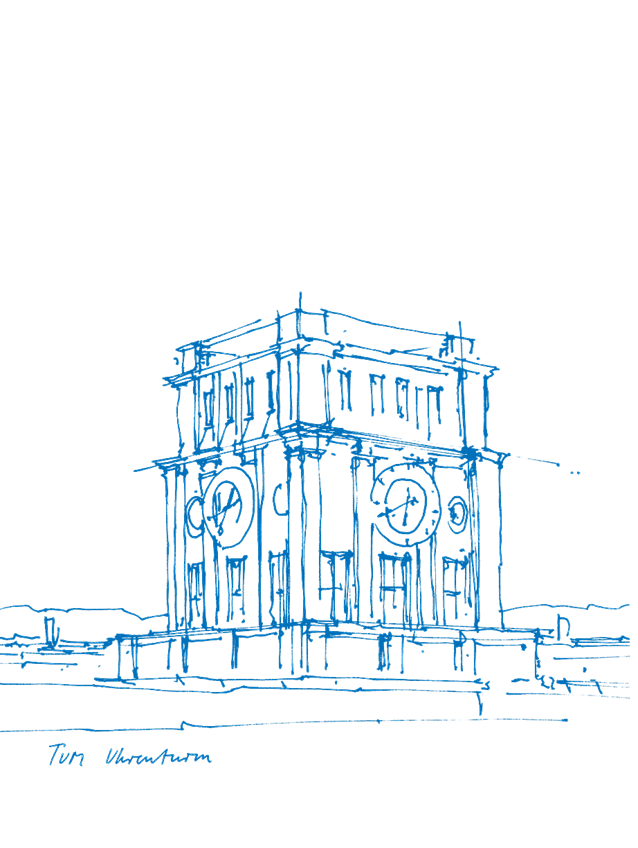
\includegraphics{../template/res/img/TUM_Uhrenturm.png}%
    \end{textblock*}%
}

\newcommand{\PraesentationStartseiteUhrenturm}{%
    \setbeamertemplate{title page}{%
        \PraesentationSeitenkopfInhalt{../template/res/img/Universitaet_Logo_RGB.pdf}%
        \PraesentationBildUhrenturm%
        \PraesentationTitelseiteInhalt%
    }%
}

\newcommand{\PraesentationStartseiteFlaggen}{%
    \setbeamertemplate{title page}{%
        \begin{textblock*}{\paperwidth}[0,1](-\PraesentationSeitenrand,\paperheight-\PraesentationSeitenrand)%
            
\includegraphics[min width=\paperwidth,max width=\paperheight,min totalsize={\paperwidth}{\paperheight},keepaspectratio,center]{../template/res/img/Universitaet_Flaggen.jpg}%
        \end{textblock*}%
        \PraesentationSeitenkopfInhalt{../template/res/img/Universitaet_Logo_weiss.pdf}%
        \PraesentationTitelseiteInhalt%
    }%
}

\newcommand{\PraesentationStartseiteLeer}{%
    \setbeamertemplate{title page}{%
        \PraesentationSeitenkopfInhalt{../template/res/img/Universitaet_Logo_weiss.pdf}%
        \PraesentationTitelseiteInhalt%
    }%
}


\newcommand{\PraesentationMasterStandard}{%
    \PraesentationFarbschemaStandard%
    \PraesentationStartseiteUhrenturm%
    \setbeamertemplate{headline}{%
        \PraesentationSeitenkopfInhalt{../template/res/img/Universitaet_Logo_RGB.pdf}%
    }%
}

\newcommand{\PraesentationMasterWeissBlau}{%
    \PraesentationFarbschemaWeissBlau%
    \PraesentationStartseiteLeer%
    \setbeamertemplate{headline}{%
        \PraesentationSeitenkopfInhalt{../template/res/img/Universitaet_Logo_weiss.pdf}%
    }%
}


\newcommand{\PraesentationMasterKopfzeileDreizeiler}{%
    \PraesentationFarbschemaStandard%
    \setbeamertemplate{title page}{%
        \begin{textblock*}{\paperwidth}[0,0](0cm, -7.8mm)%
            \color{TUMBlau}\PraesentationSchriftgroesseDreizeiler\selectfont%
            \LehrstuhlName\\%
            \FakultaetName\\%
            \UniversitaetName\vskip0pt%
            \normalcolor\normalsize\selectfont%
        \end{textblock*}%
        \PraesentationSeitenkopfInhalt{../template/res/img/Universitaet_Logo_RGB.pdf}%
        \PraesentationBildUhrenturm%
        \PraesentationTitelseiteInhalt%
    }%
    \setbeamertemplate{headline}{%
        \begin{textblock*}{\paperwidth}[0,0](0cm, 0cm)%
            \begin{minipage}[t][2cm][t]{\paperwidth}%
                \color{TUMBlau}\PraesentationSchriftgroesseDreizeiler\selectfont%
                \LehrstuhlName\\[1.38mm]%
                \FakultaetName\\[1.44mm]%
                \UniversitaetName\vskip0pt%
                \normalcolor\normalsize\selectfont%
            \end{minipage}%
        \end{textblock*}%
        \PraesentationSeitenkopfInhalt{../template/res/img/Universitaet_Logo_RGB.pdf}%
    }%
}

\newcommand{\PraesentationMasterWeissSchwarz}{%
    \PraesentationFarbschemaWeissSchwarz%
    \setbeamertemplate{title page}{%
        \PraesentationTitelseiteInhalt%
        \PraesentationSeitenkopfInhalt{../template/res/img/Universitaet_Logo_weiss.pdf}%
    }
    \setbeamertemplate{headline}{%
        \PraesentationSeitenkopfInhalt{../template/res/img/Universitaet_Logo_weiss.pdf}%
    }
}

\newcommand{\PraesentationTitelseite}{\frame[plain]{\titlepage}}
\newcommand{\PraesentationUeberschriftZweizeilig}[2]{\frametitle{#1\\[8mm]#2}}

\setbeamersize{
    text margin left=\PraesentationSeitenrand,
    text margin right=\PraesentationSeitenrand
}

\setbeamertemplate{frametitle}{%
    {\rule{0pt}{42mm + \PraesentationPositionKorrekturOben}\PraesentationSchriftgroesseSehrGross\selectfont\insertframetitle\newline\vspace*{-6.7mm}}%
}

% Aufzählungen:
\newcommand{\PraesentationAufzaehlungEbeneEinsSymbol}{\raise2pt\hbox{\donotcoloroutermaths\usebeamercolor{itemize subitem}\PraesentationSchriftgroesseAufzaehlungszeichen$\bullet$}}
\newcommand{\PraesentationAufzaehlungEbeneZweiSymbol}{\raise1.25pt\hbox{\donotcoloroutermaths\usebeamercolor{itemize subitem}$-$}}
\setbeamertemplate{itemize items}[circle]
\setbeamertemplate{itemize subitem}[triangle]
\setbeamercolor{itemize subitem}{fg=black}
\setbeamerfont{itemize/enumerate subbody}{size=\normalsize}
\setbeamertemplate{itemize item}{\PraesentationAufzaehlungEbeneEinsSymbol}
\setbeamertemplate{itemize subitem}{\PraesentationAufzaehlungEbeneZweiSymbol{}}
%\addtolength{\leftmarginii}{16mm-2pt}%

\newenvironment{PraesentationAufzaehlung}
{%
    \vspace{-\baselineskip}%
    \begin{itemize}%
        \setlength{\itemsep}{0pt}%
        \setlength{\parskip}{0pt}%
        \setlength{\parsep}{0pt}%
        \addtolength{\itemindent}{-1ex}%
}{%
    \end{itemize}%
}

%%%%%%%%%%%%%%%%%%%%%%%%%%%%%%%%%%%%%%%%%%%%%%%%%%%%%%%%%%%%%%%%%%%%%%%%%%%%%%%%
% DOKUMENT
%%%%%%%%%%%%%%%%%%%%%%%%%%%%%%%%%%%%%%%%%%%%%%%%%%%%%%%%%%%%%%%%%%%%%%%%%%%%%%%%


% PDF-Einstellungen:
\hypersetup{
    pdfstartview={Fit},
    pdfproducer={\AllgemeinErsteller},
    pdfcreator={\AllgemeinGestalter}
}

\textblockorigin{\PraesentationSeitenrand}{\PraesentationSeitenrand} % Ursprung für Positionierung

\setbeamerfont{footnote}{size=\PraesentationSchriftgroesseKlein}

\setbeamertemplate{footline}{
    \hbox{%
        \usebeamerfont{footnote}%
        \begin{beamercolorbox}[wd=.9\paperwidth]{}%
            \hspace*{\PraesentationSeitenrand}%
            \PersonTitel{} \PersonVorname~\PersonNachname~(\UniversitaetAbkuerzung) \PraesentationFusszeileZusatz{}%
        \end{beamercolorbox}%
        \begin{beamercolorbox}[wd=.1\paperwidth]{}%
            \insertframenumber{}%
            \raggedleft
            \hspace*{\PraesentationSeitenrand}%
        \end{beamercolorbox}%
        \vspace*{3.25mm}%
    }%
}

\setbeamertemplate{navigation symbols}{}
 % !!! NICHT ENTFERNEN !!!
%%%%%%%%%%%%%%%%%%%%%%%%%%%%%%%%%%%%%%%%%%%%%%%%%%%%%%%%%%%%%%%%%%%%%%%%%%%%%%%%
\begin{document}
\setlength{\baselineskip}{\PraesentationAbstandAbsatz}
\setlength{\parskip}{\baselineskip}

%%%%%%%%%%%%%%%%%%%%%%%%%%%%%%%%%%%%%%%%%%%%%%%%%%%%%%%%%%%%%%%%%%%%%%%%%%%%%%%%
% FOLIENSTIL: Standard
% !!!ÄNDERUNG HIER:!!!
\PraesentationMasterStandard

\PraesentationTitelseite % Fügt die Startseite ein

\begin{frame}
	\frametitle{Hausaufgabe 1}
	\vspace{0.25cm}

	\begin{multicols}{2}
		Formulieren Sie die folgenden Anfragen auf dem bekannten Unischema in SQL:
		\begin{enumerate}[a)]
			\item Finden Sie die \textit{Studenten}, die Sokrates aus \textit{Vorlesung(en)} kennen.
			\item Finden Sie die Studenten, die Vorlesungen hören, die auch Fichte hört.
			% \item Finden Sie die Assistenten von Professoren, die den Studenten Fichte unterrichtet haben – z.B. als potentielle Betreuer seiner Diplomarbeit.
			% \item Geben Sie die Namen der Professoren an, die Xenokrates aus Vorlesungen kennt.
			% \item Welche Vorlesungen werden von Studenten im Grundstudium (1.-4. Semester) gehört? \\
			%       Geben Sie die Titel dieser Vorlesungen an.
		\end{enumerate}
		\vfill\columnbreak

		\begin{center}
			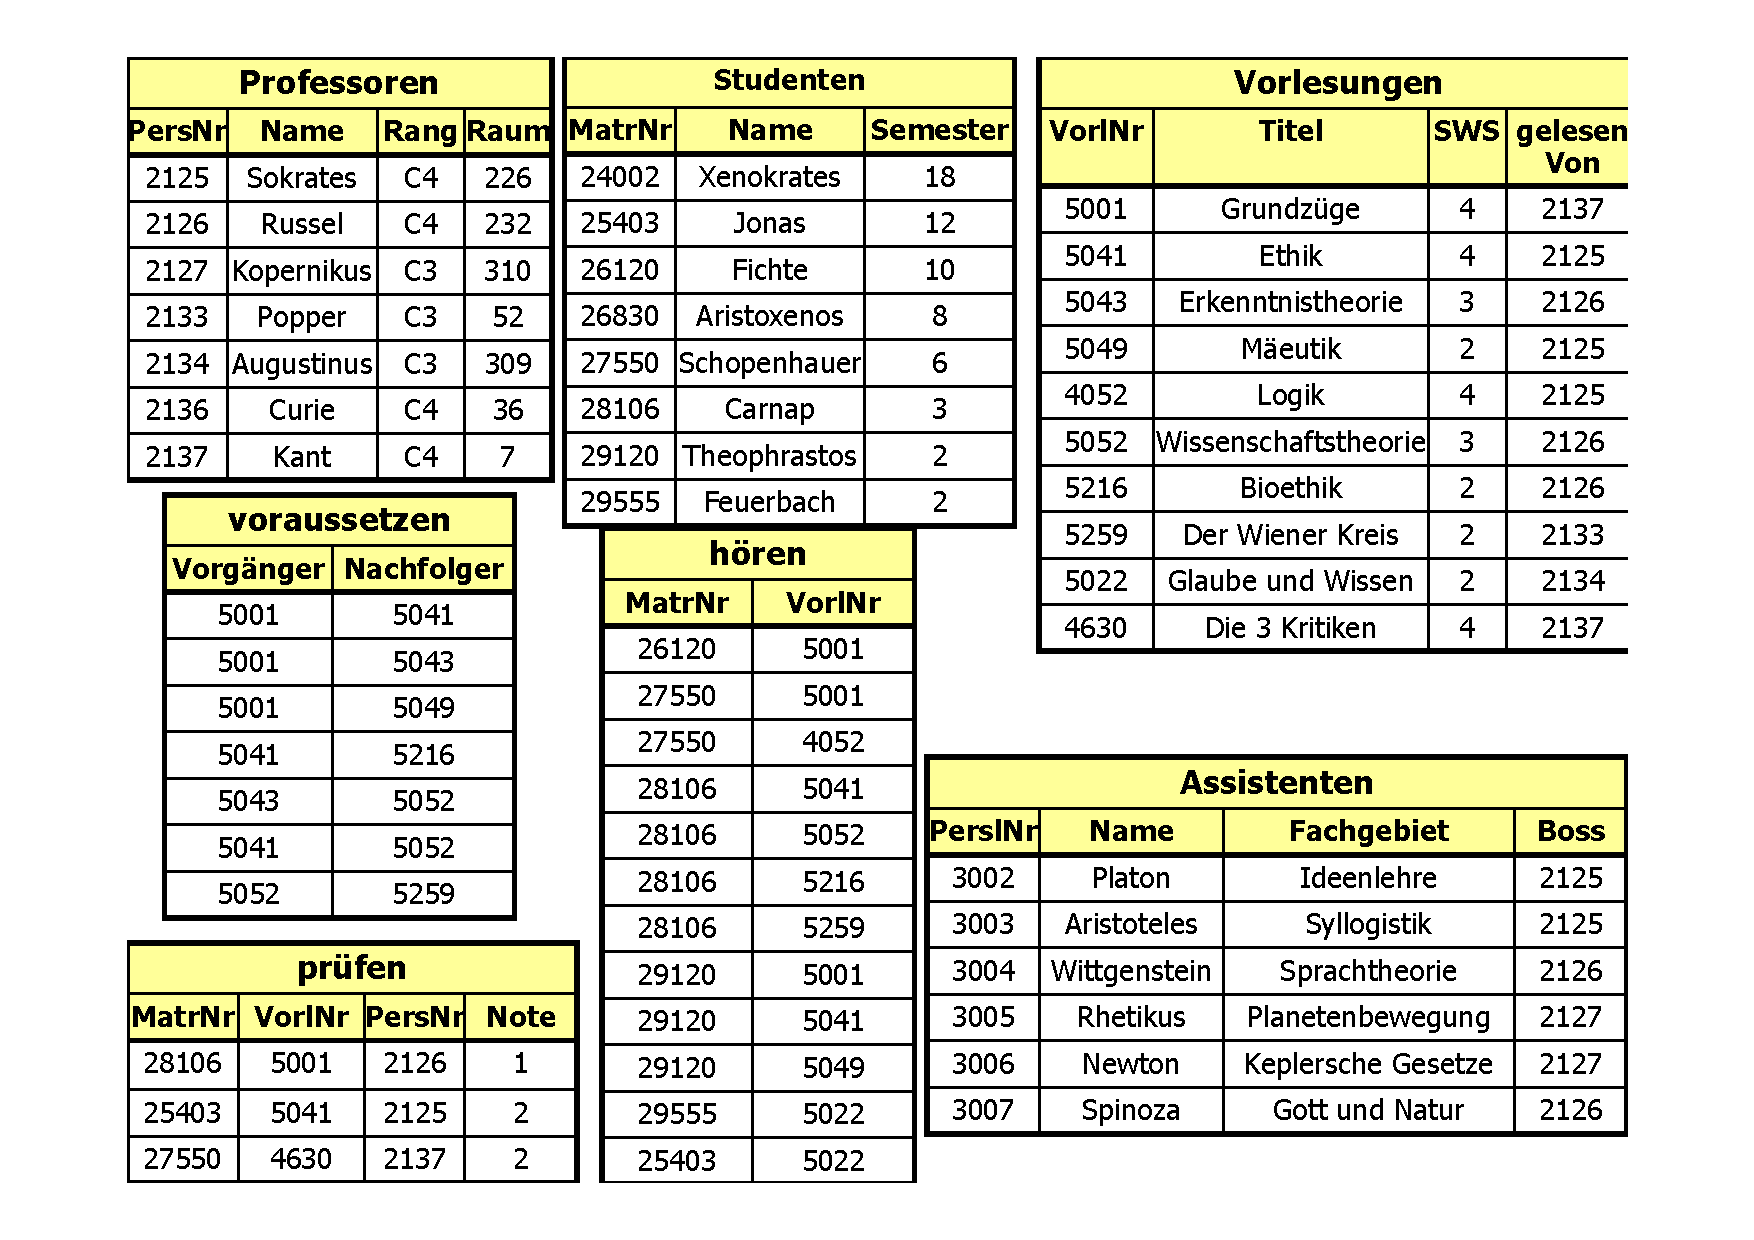
\includegraphics[height=.6\paperheight]{../img/uni.pdf}
		\end{center}

	\end{multicols}
\end{frame}

\begin{frame}[fragile]
	\frametitle{Hausaufgabe 1}
	\vspace{0.25cm}

	\begin{multicols}{2}
		Formulieren Sie die folgenden Anfragen auf dem bekannten Unischema in SQL:
		\begin{enumerate}[a)]
			\item Finden Sie die \textit{Studenten}, die Sokrates aus \textit{Vorlesung(en)} kennen.
			% \item Finden Sie die Studenten, die Vorlesungen hören, die auch Fichte hört.
			% \item Finden Sie die Assistenten von Professoren, die den Studenten Fichte unterrichtet haben – z.B. als potentielle Betreuer seiner Diplomarbeit.
			% \item Geben Sie die Namen der Professoren an, die Xenokrates aus Vorlesungen kennt.
			% \item Welche Vorlesungen werden von Studenten im Grundstudium (1.-4. Semester) gehört? \\
			%       Geben Sie die Titel dieser Vorlesungen an.
		\end{enumerate}

		\begin{minted}{sql}
SELECT s.Name, s.MatrNr
FROM Studenten s, hoeren h, Vorlesungen v, 
     Professoren p
WHERE s.MatrNr = h.MatrNr
  AND h.VorlNr = v.VorlNr
  AND v.gelesenVon = p.PersNr
  AND p.Name = 'Sokrates';
/* Es kann DISTINCT verwendet werden, 
   um Duplikate zu vermeiden */
		\end{minted}
		\vfill\columnbreak

		\begin{center}
			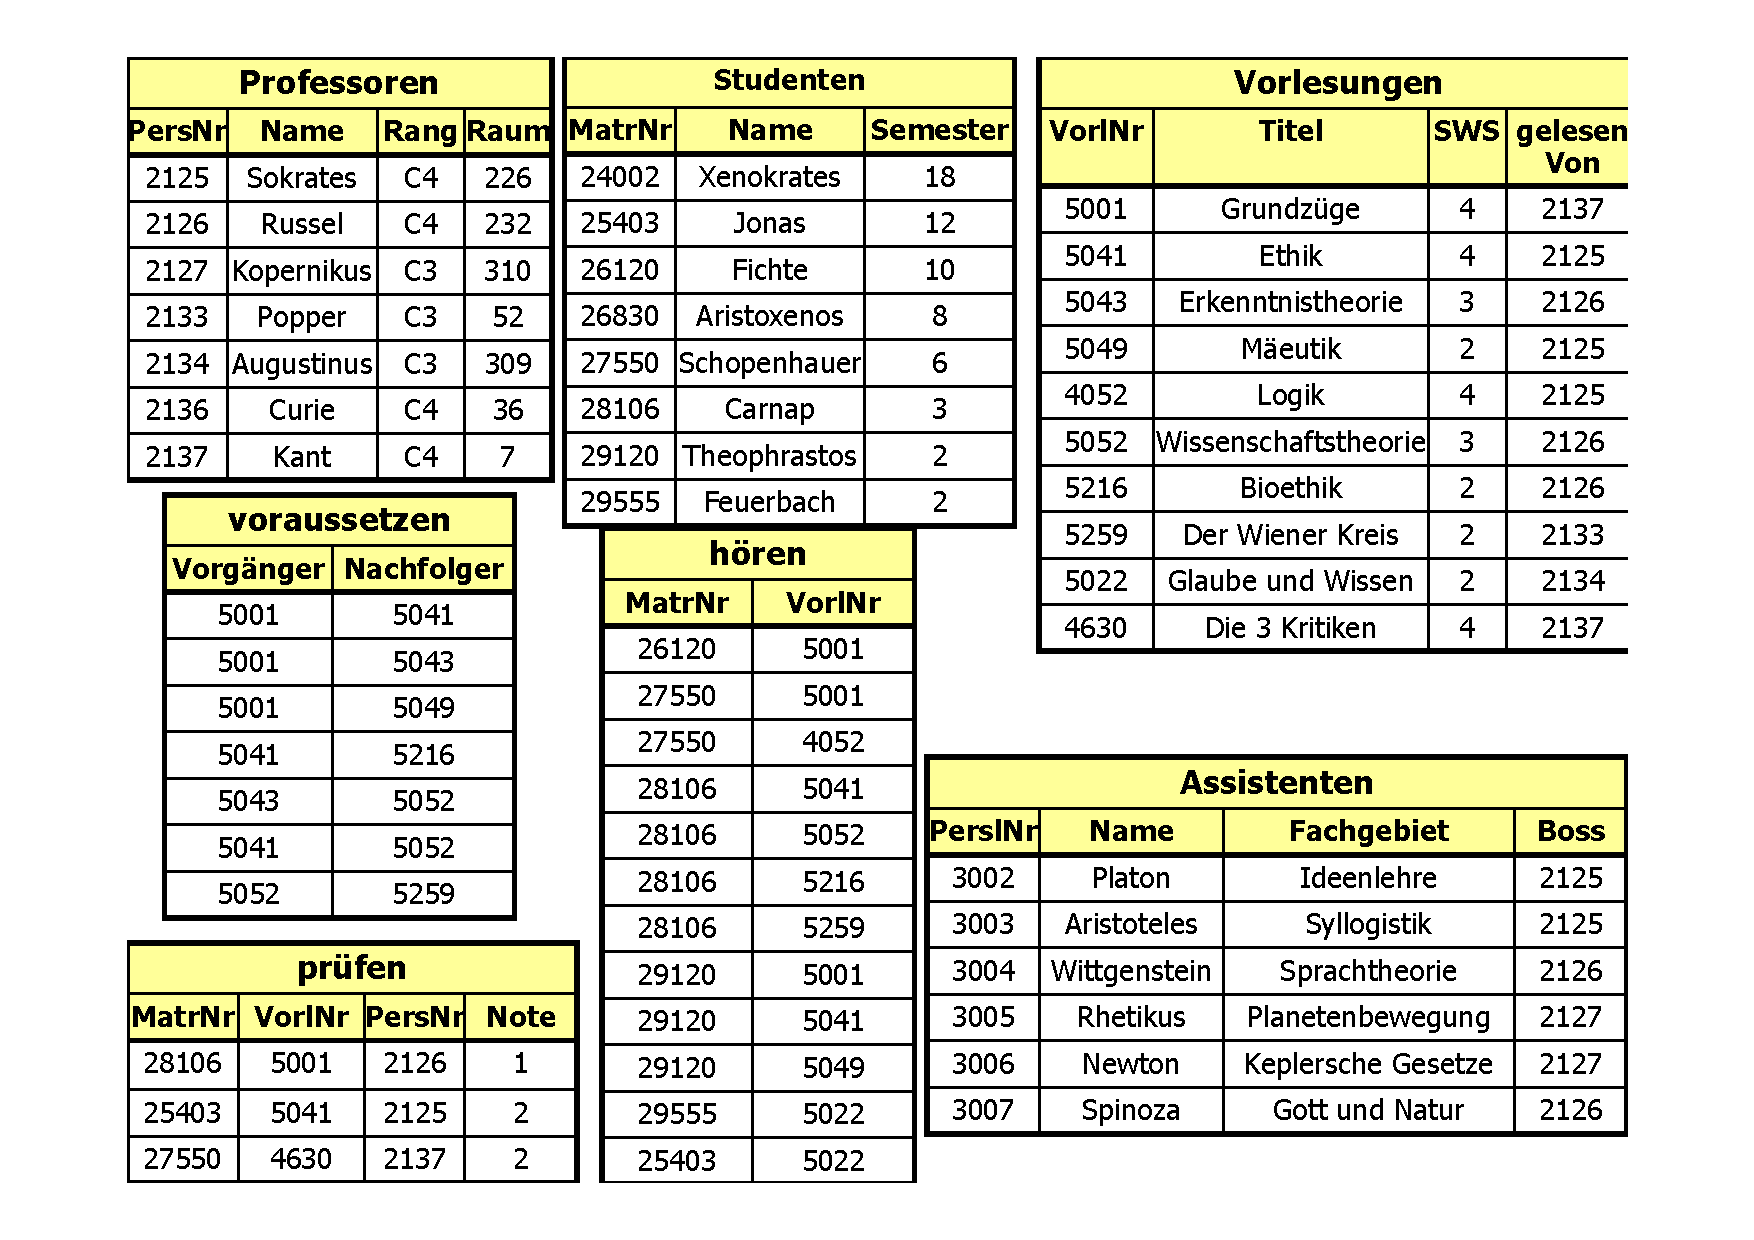
\includegraphics[height=.6\paperheight]{../img/uni.pdf}
		\end{center}
	\end{multicols}
\end{frame}

\begin{frame}[fragile]
	\frametitle{Hausaufgabe 1}
	\vspace{0.25cm}

	\begin{multicols}{2}
		Formulieren Sie die folgenden Anfragen auf dem bekannten Unischema in SQL:
		\begin{enumerate}[b)]
			% \item Finden Sie die \textit{Studenten}, die Sokrates aus \textit{Vorlesung(en)} kennen.
			\item Finden Sie die Studenten, die Vorlesungen hören, die auch Fichte hört.
			% \item Finden Sie die Assistenten von Professoren, die den Studenten Fichte unterrichtet haben – z.B. als potentielle Betreuer seiner Diplomarbeit.
			% \item Geben Sie die Namen der Professoren an, die Xenokrates aus Vorlesungen kennt.
			% \item Welche Vorlesungen werden von Studenten im Grundstudium (1.-4. Semester) gehört? \\
			%       Geben Sie die Titel dieser Vorlesungen an.
		\end{enumerate}

		\begin{minted}{sql}
SELECT DISTINCT s1.Name, s1.MatrNr
FROM Studenten s1, Studenten s2, 
	 hoeren h1, hoeren h2
WHERE s1.MatrNr = h1.MatrNr
  AND s1.MatrNr != s2.MatrNr
  AND s2.MatrNr = h2.MatrNr
  AND h1.VorlNr = h2.VorlNr
  AND s2.Name = 'Fichte';
		\end{minted}
		\vfill\columnbreak

		\begin{center}
			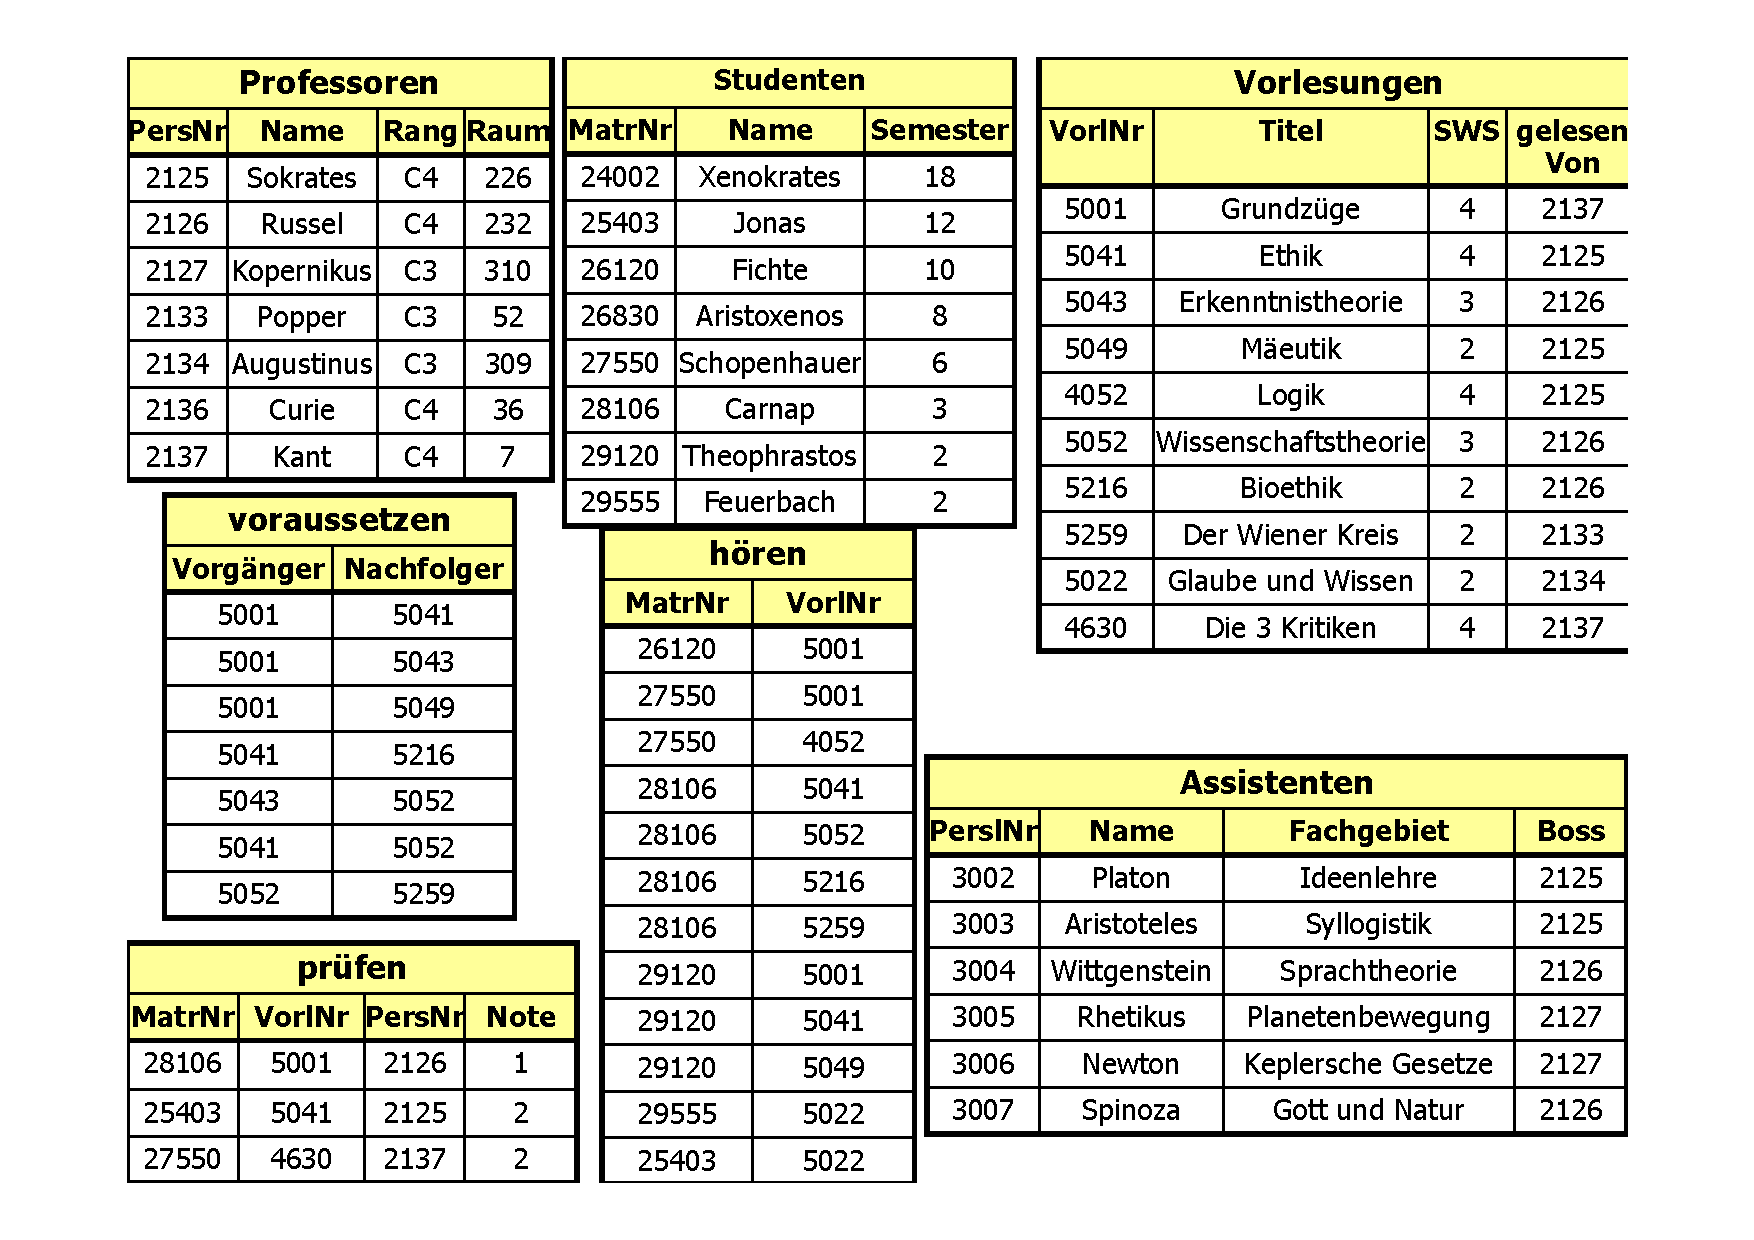
\includegraphics[height=.6\paperheight]{../img/uni.pdf}
		\end{center}
	\end{multicols}
\end{frame}

\begin{frame}[fragile]
	\frametitle{Hausaufgabe 1}
	\vspace{0.25cm}

	\begin{multicols}{2}
		Formulieren Sie die folgenden Anfragen auf dem bekannten Unischema in SQL:
		\begin{enumerate}[a)]
			\setcounter{enumi}{2}
			% \item Finden Sie die \textit{Studenten}, die Sokrates aus \textit{Vorlesung(en)} kennen.
			% \item Finden Sie die Studenten, die Vorlesungen hören, die auch Fichte hört.
			\item Finden Sie die Assistenten von Professoren, die den Studenten Fichte unterrichtet haben – z.B. als potentielle Betreuer seiner Diplomarbeit.
			\item Geben Sie die Namen der Professoren an, die Xenokrates aus Vorlesungen kennt.
			% \item Welche Vorlesungen werden von Studenten im Grundstudium (1.-4. Semester) gehört? \\
			%       Geben Sie die Titel dieser Vorlesungen an.
		\end{enumerate}
		\vfill\columnbreak

		\begin{center}
			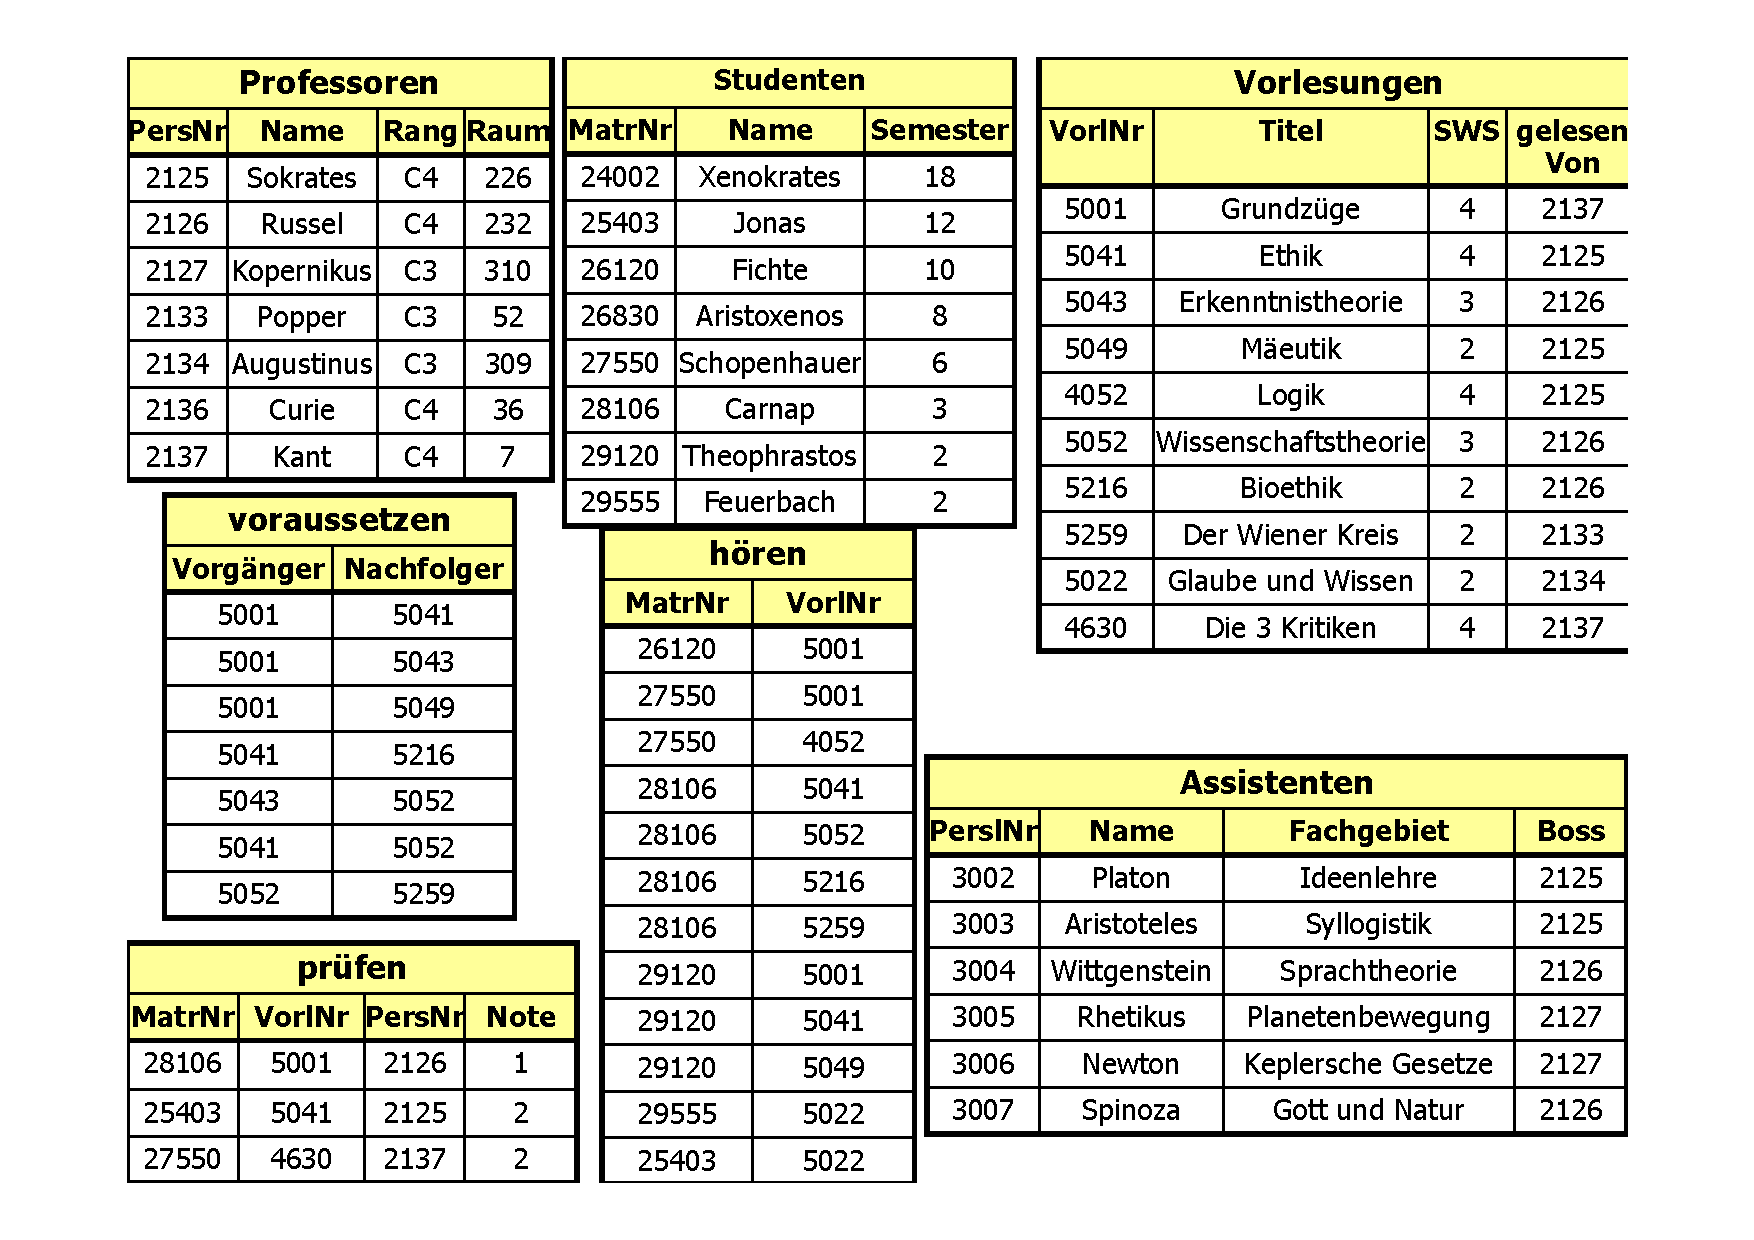
\includegraphics[height=.6\paperheight]{../img/uni.pdf}
		\end{center}
	\end{multicols}
\end{frame}

\begin{frame}[fragile]
	\frametitle{Hausaufgabe 1}
	\vspace{0.25cm}

	\begin{multicols}{2}
		Formulieren Sie die folgenden Anfragen auf dem bekannten Unischema in SQL:
		\begin{enumerate}[a)]
			\setcounter{enumi}{2}
			% \item Finden Sie die \textit{Studenten}, die Sokrates aus \textit{Vorlesung(en)} kennen.
			% \item Finden Sie die Studenten, die Vorlesungen hören, die auch Fichte hört.
			\item Finden Sie die Assistenten von Professoren, die den Studenten Fichte unterrichtet haben – z.B. als potentielle Betreuer seiner Diplomarbeit.
			% \item Geben Sie die Namen der Professoren an, die Xenokrates aus Vorlesungen kennt.
			% \item Welche Vorlesungen werden von Studenten im Grundstudium (1.-4. Semester) gehört? \\
			%       Geben Sie die Titel dieser Vorlesungen an.
		\end{enumerate}
		\begin{minted}{sql}
SELECT a.Name, a.PersNr
FROM Assistenten a, Professoren p, Vorlesungen v, 
	 hoeren h, Studenten s
WHERE a.Boss = p.PersNr
  AND p.PersNr = v.gelesenVon
  AND v.VorlNr = h.VorlNr
  AND h.MatrNr = s.MatrNr
  AND s.Name = 'Fichte';
		\end{minted}
		\vfill\columnbreak

		\begin{center}
			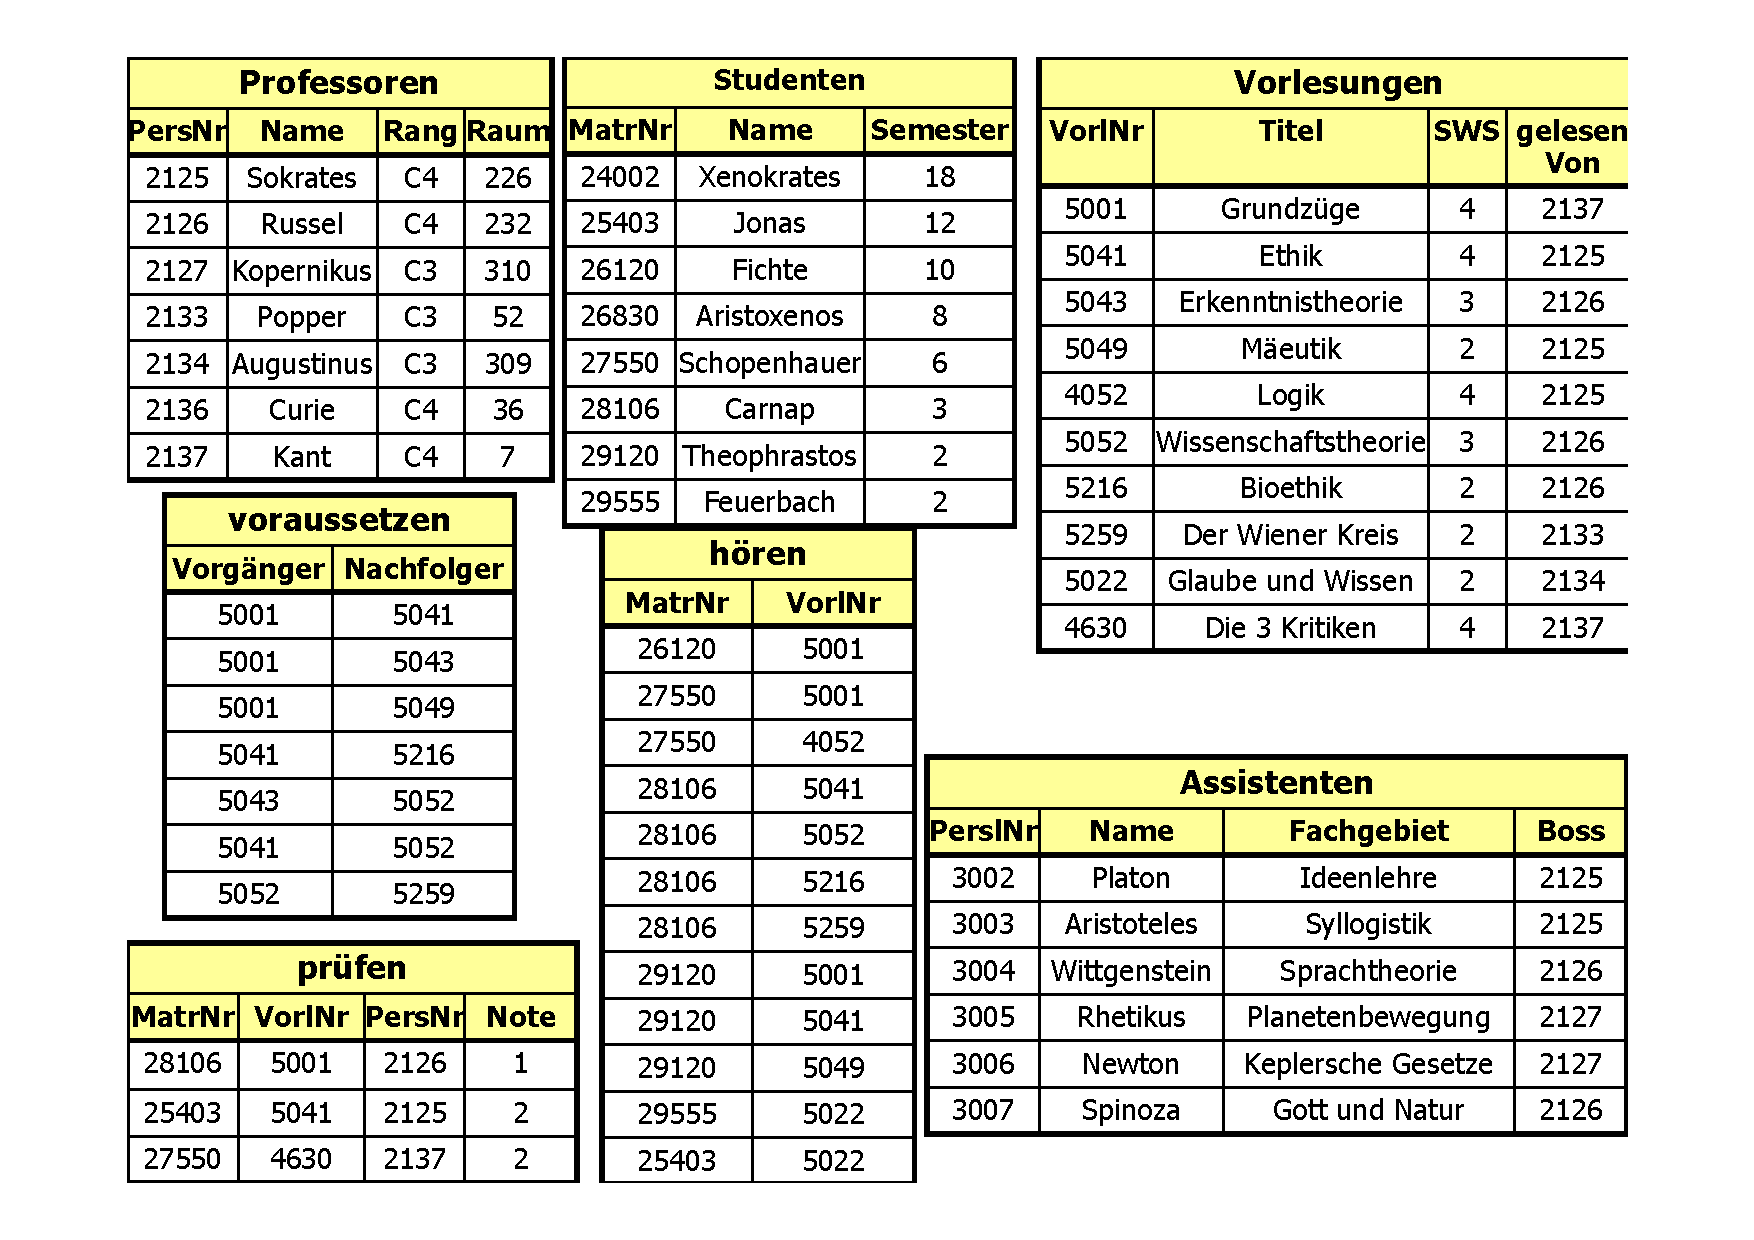
\includegraphics[height=.6\paperheight]{../img/uni.pdf}
		\end{center}
	\end{multicols}
\end{frame}

\begin{frame}[fragile]
	\frametitle{Hausaufgabe 1}
	\vspace{0.25cm}

	\begin{multicols}{2}
		Formulieren Sie die folgenden Anfragen auf dem bekannten Unischema in SQL:
		\begin{enumerate}[a)]
			\setcounter{enumi}{3}
			% \item Finden Sie die \textit{Studenten}, die Sokrates aus \textit{Vorlesung(en)} kennen.
			% \item Finden Sie die Studenten, die Vorlesungen hören, die auch Fichte hört.
			% \item Finden Sie die Assistenten von Professoren, die den Studenten Fichte unterrichtet haben – z.B. als potentielle Betreuer seiner Diplomarbeit.
			\item Geben Sie die Namen der Professoren an, die Xenokrates aus Vorlesungen kennt.
			% \item Welche Vorlesungen werden von Studenten im Grundstudium (1.-4. Semester) gehört? \\
			%       Geben Sie die Titel dieser Vorlesungen an.
		\end{enumerate}
		\begin{minted}{sql}
SELECT p.PersNr, p.Name
FROM Professoren p, hoeren h, Vorlesungen v,
	 Studenten s
WHERE p.PersNr = v.gelesenVon
  AND v.VorlNr = h.VorlNr
  AND h.MatrNr = s.MatrNr
  AND s.Name = 'Xenokrates';
		\end{minted}
		\vfill\columnbreak

		\begin{center}
			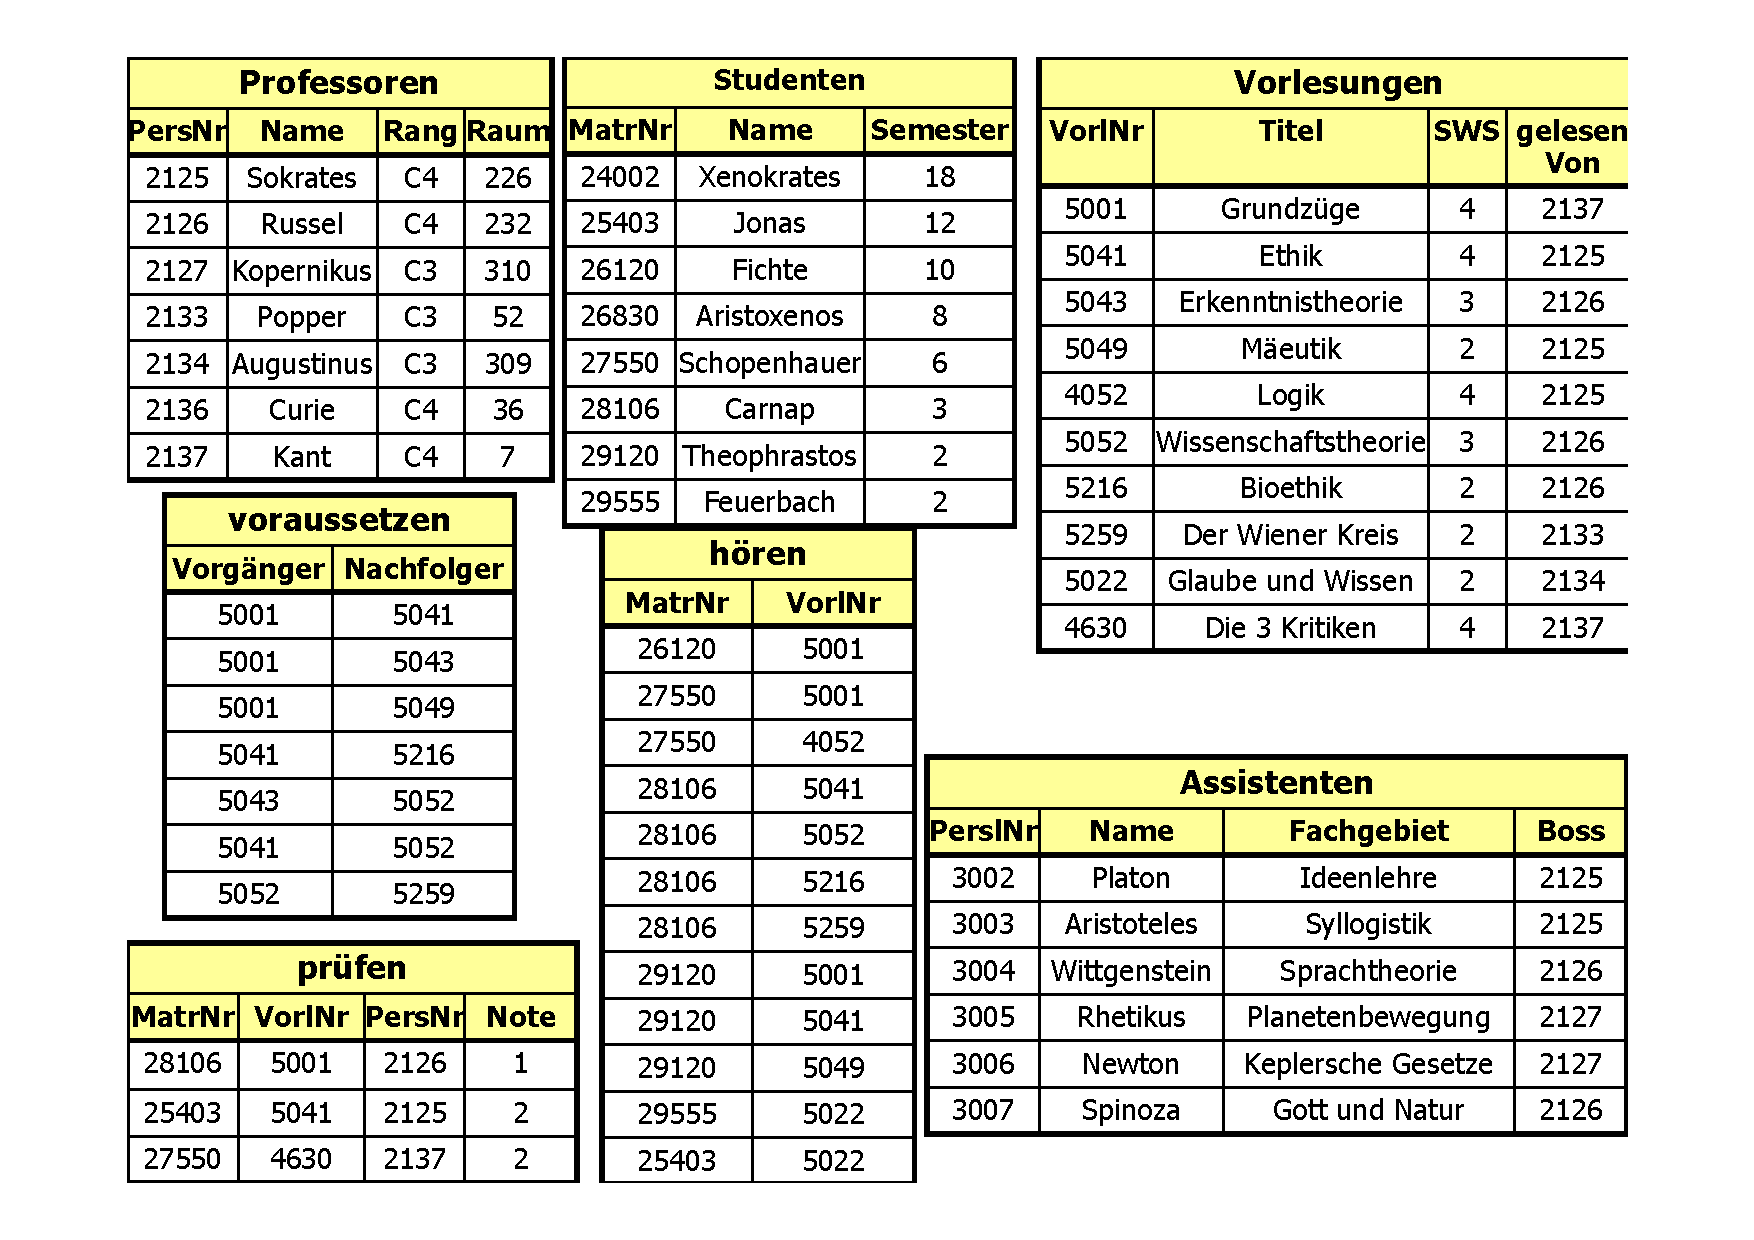
\includegraphics[height=.6\paperheight]{../img/uni.pdf}
		\end{center}
	\end{multicols}
\end{frame}

\begin{frame}[fragile]
	\frametitle{Hausaufgabe 1}
	\vspace{0.25cm}

	\begin{multicols}{2}
		Formulieren Sie die folgenden Anfragen auf dem bekannten Unischema in SQL:
		\begin{enumerate}[a)]
			\setcounter{enumi}{4}
			% \item Finden Sie die \textit{Studenten}, die Sokrates aus \textit{Vorlesung(en)} kennen.
			% \item Finden Sie die Studenten, die Vorlesungen hören, die auch Fichte hört.
			% \item Finden Sie die Assistenten von Professoren, die den Studenten Fichte unterrichtet haben – z.B. als potentielle Betreuer seiner Diplomarbeit.
			% \item Geben Sie die Namen der Professoren an, die Xenokrates aus Vorlesungen kennt.
			\item Welche Vorlesungen werden von Studenten im Grundstudium (1.-4. Semester) gehört? \\
			      Geben Sie die Titel dieser Vorlesungen an.
		\end{enumerate}
		\vfill\columnbreak

		\begin{center}
			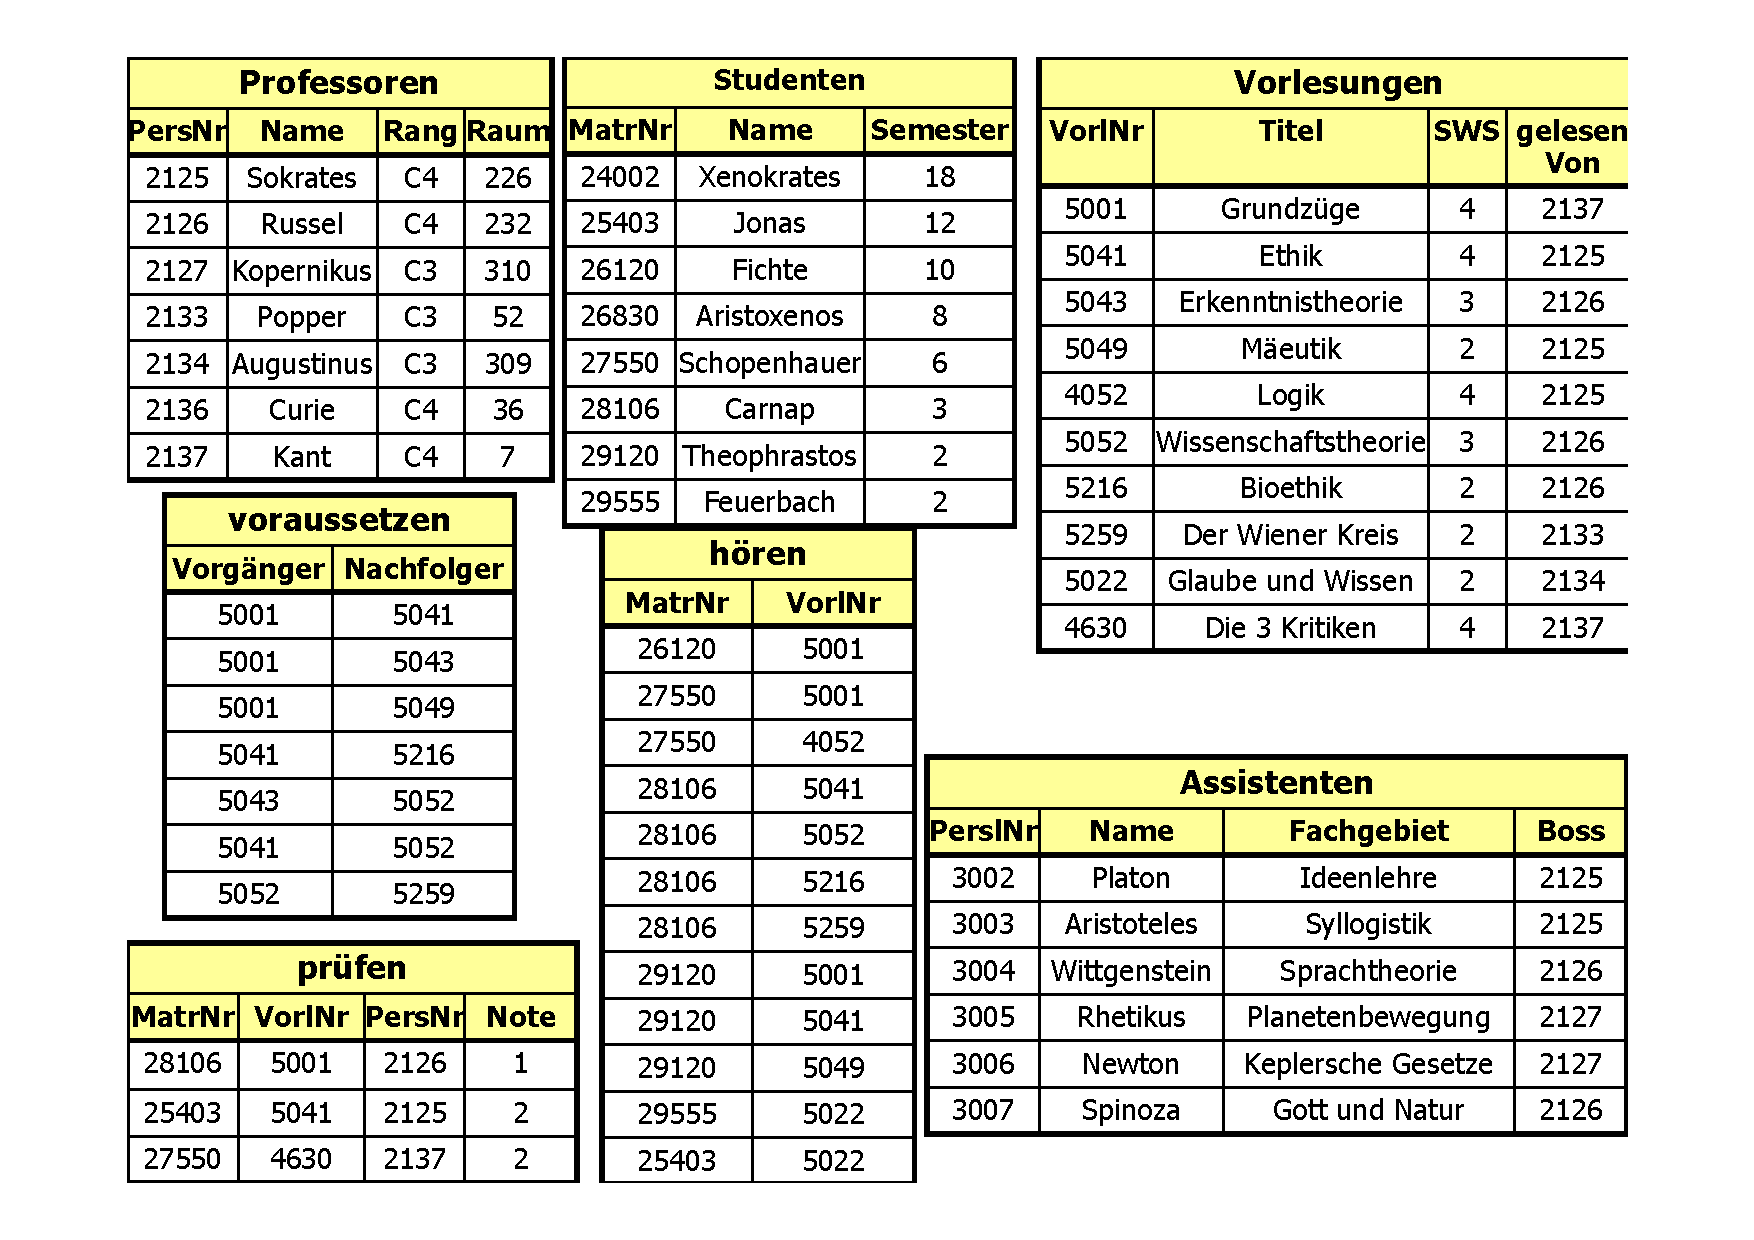
\includegraphics[height=.6\paperheight]{../img/uni.pdf}
		\end{center}
	\end{multicols}
\end{frame}

\begin{frame}[fragile]
	\frametitle{Hausaufgabe 1}
	\vspace{0.25cm}

	\begin{multicols}{2}
		Formulieren Sie die folgenden Anfragen auf dem bekannten Unischema in SQL:
		\begin{enumerate}[a)]
			\setcounter{enumi}{4}
			% \item Finden Sie die \textit{Studenten}, die Sokrates aus \textit{Vorlesung(en)} kennen.
			% \item Finden Sie die Studenten, die Vorlesungen hören, die auch Fichte hört.
			% \item Finden Sie die Assistenten von Professoren, die den Studenten Fichte unterrichtet haben – z.B. als potentielle Betreuer seiner Diplomarbeit.
			% \item Geben Sie die Namen der Professoren an, die Xenokrates aus Vorlesungen kennt.
			\item Welche Vorlesungen werden von Studenten im Grundstudium (1.-4. Semester) gehört? \\
			      Geben Sie die Titel dieser Vorlesungen an.
		\end{enumerate}
		\begin{minted}{sql}
SELECT v.Titel
FROM Vorlesungen v, hoeren h, Studenten s
WHERE v.VorlNr = h.VorlNr
  AND h.MatrNr = s.MatrNr
  AND s.Semester BETWEEN 1 AND 4;
/* BETWEEN: Anfang / Ende inklusiv */
		\end{minted}
		\vfill\columnbreak

		\begin{center}
			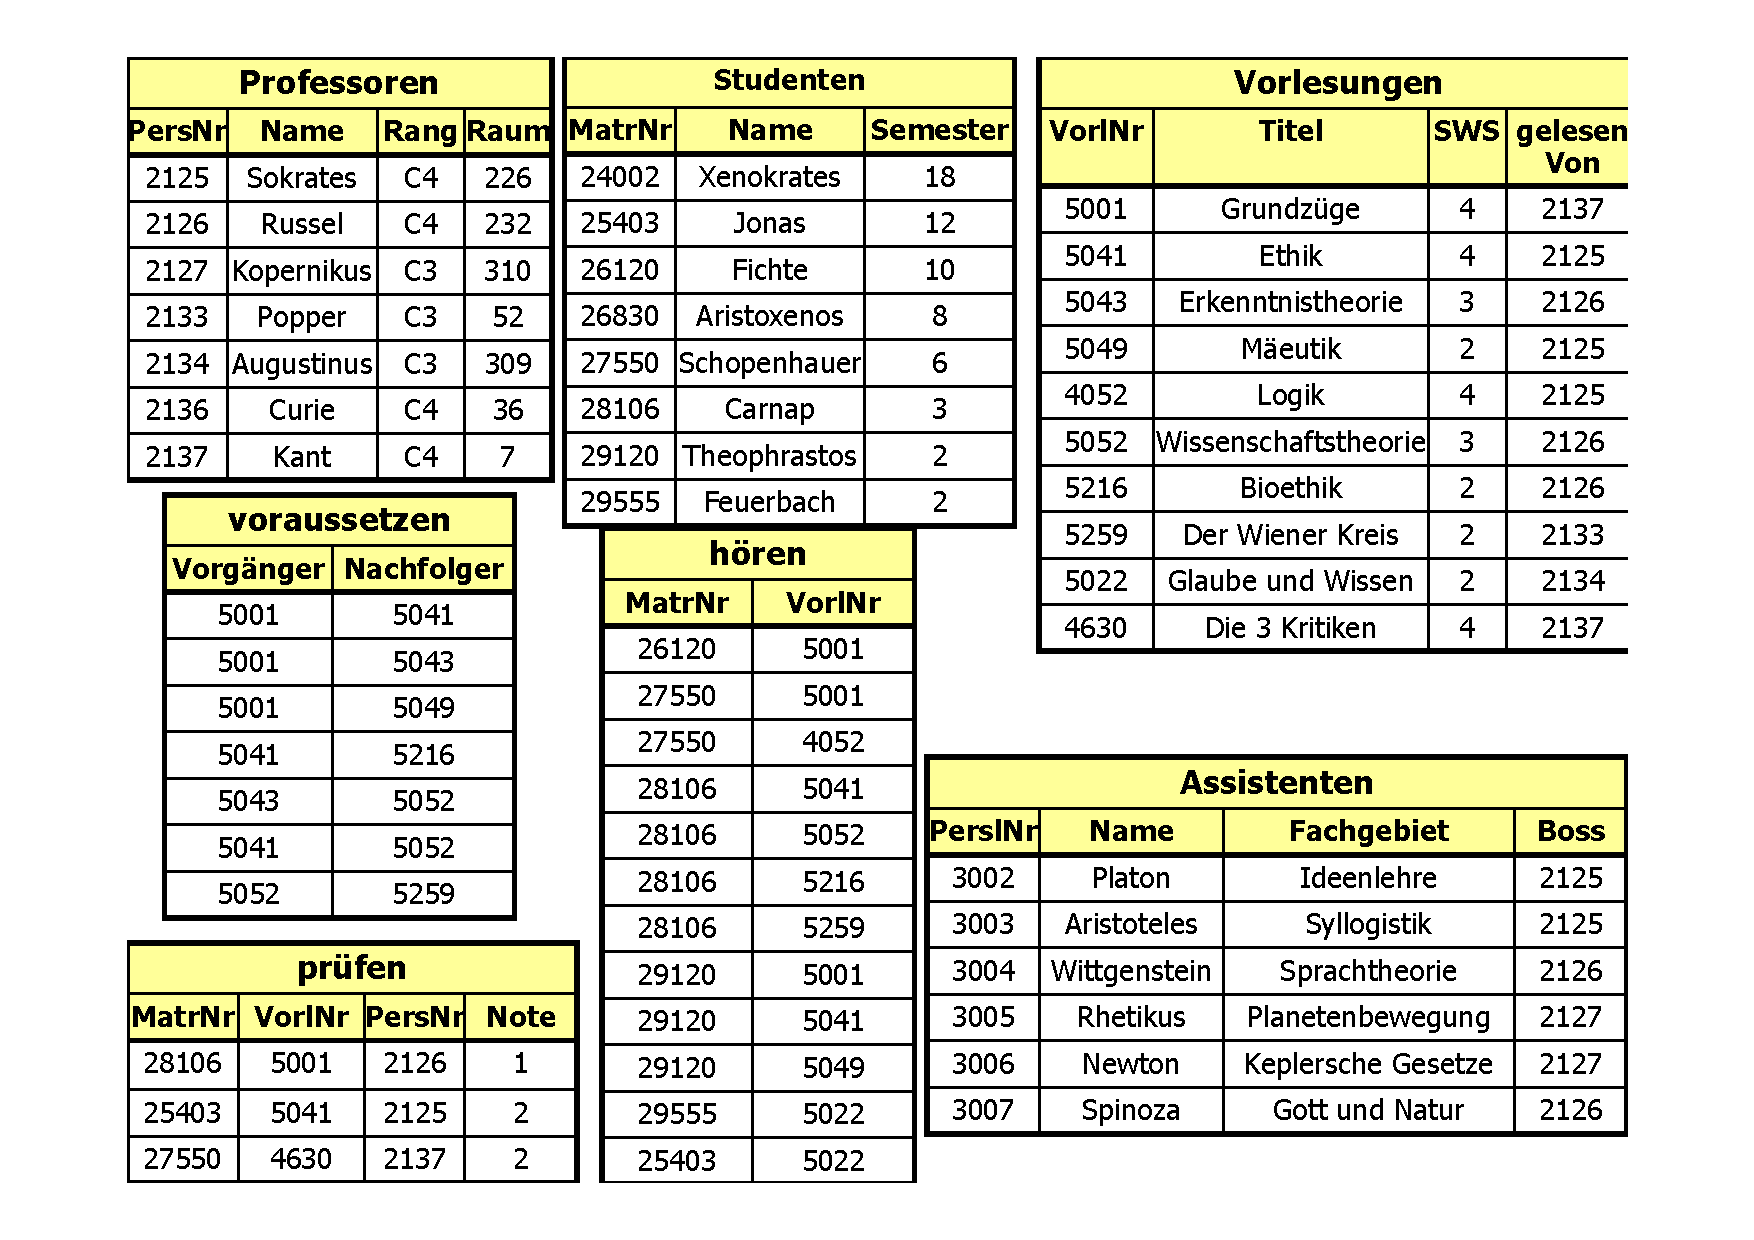
\includegraphics[height=.6\paperheight]{../img/uni.pdf}
		\end{center}
	\end{multicols}
\end{frame}

\begin{frame}
	\frametitle{Hausaufgabe 2}
	\vspace{0.25cm}

	\begin{multicols}{2}
		Formulieren Sie die folgenden Anfragen auf dem bekannten Unischema in SQL:
		\begin{enumerate}[a)]
			\item Bestimmen Sie das durchschnittliche Semester der Studenten der Universität.
			\item Bestimmen Sie das durchschnittliche Semester der Studenten, die mindestens eine Vorlesung bei Sokrates hören.
			% \item Bestimmen Sie, wie viele Vorlesungen im Schnitt pro Student gehört werden. 
			% 	  Beachten Sie, dass Studenten, die keine Vorlesung hören, in das Ergebnis einfließen müssen.
		\end{enumerate}
		\vfill\columnbreak

		\begin{center}
			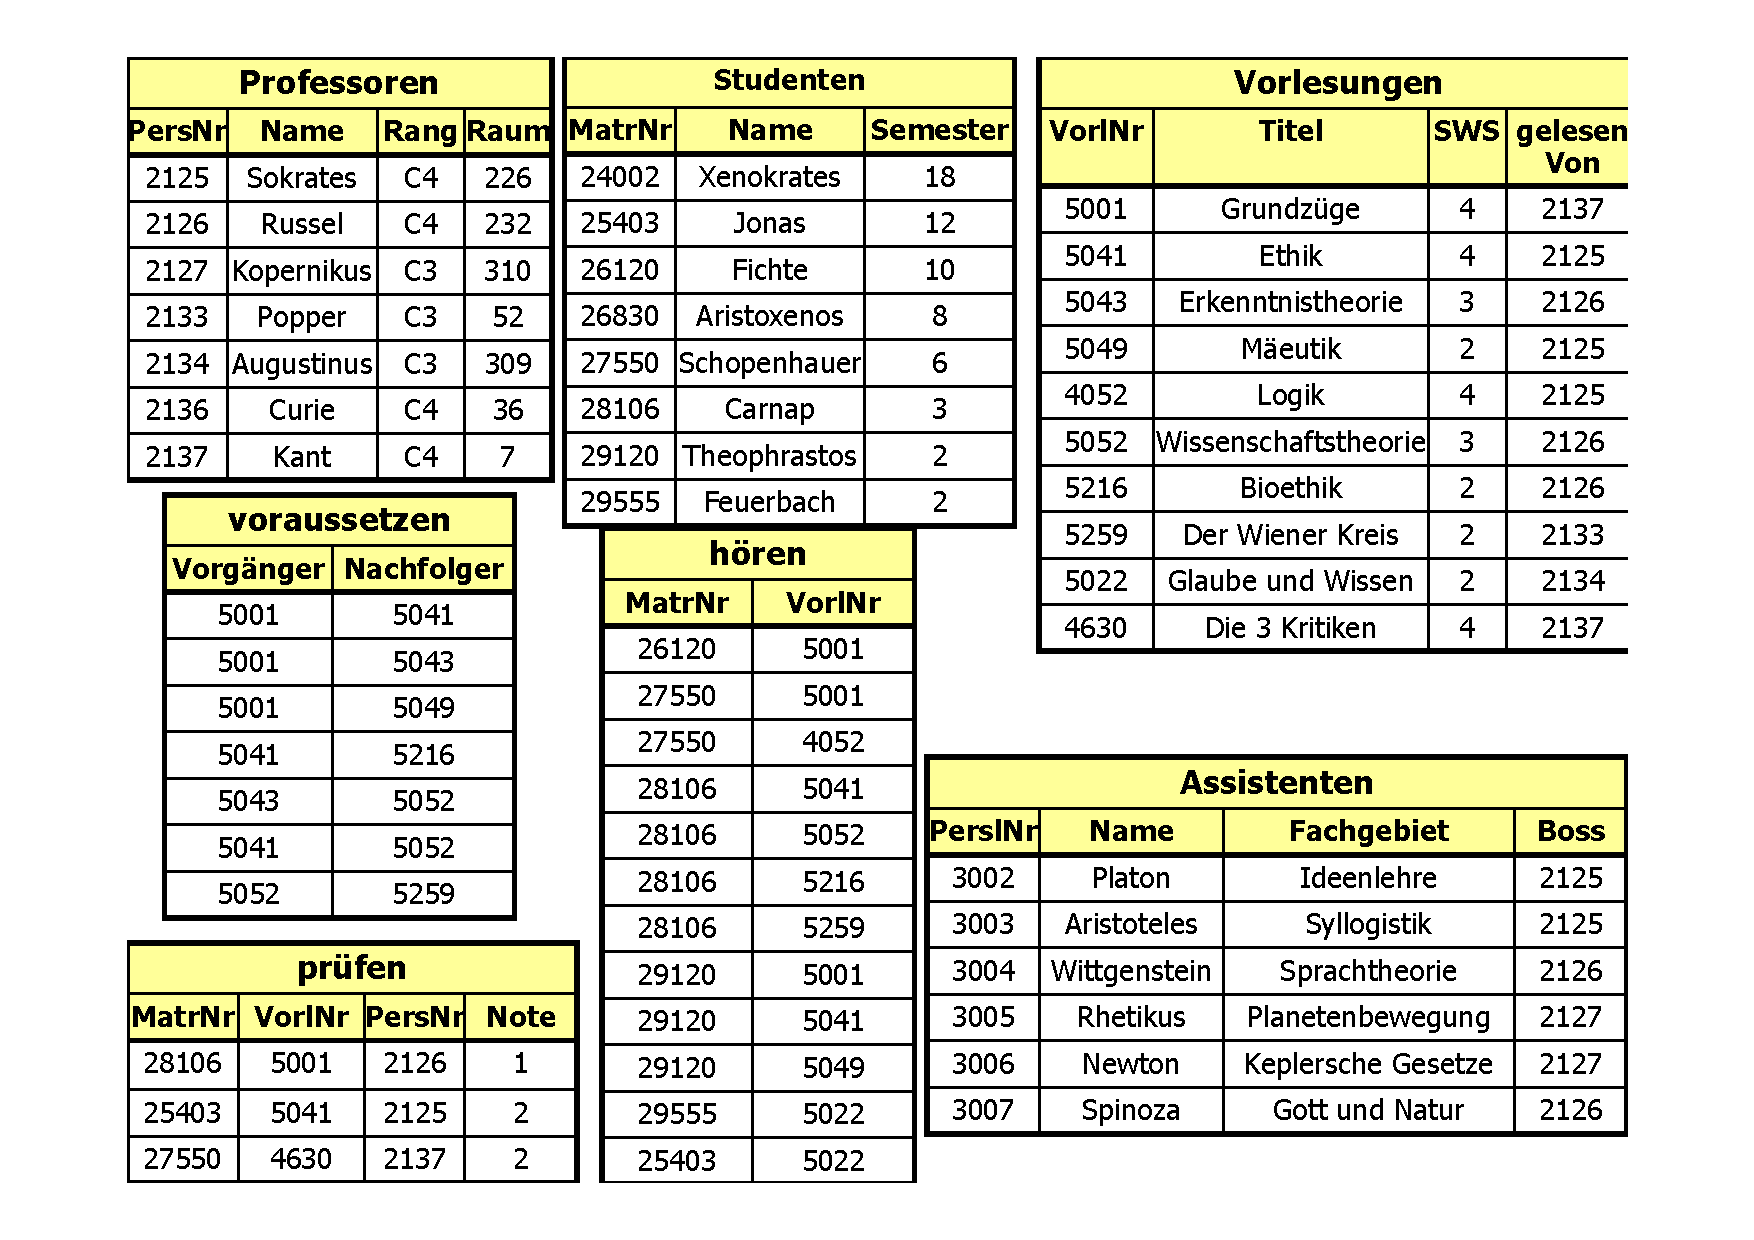
\includegraphics[height=.6\paperheight]{../img/uni.pdf}
		\end{center}
	\end{multicols}
\end{frame}

\begin{frame}[fragile]
	\frametitle{Hausaufgabe 2}
	\vspace{0.25cm}

	\begin{multicols}{2}
		Formulieren Sie die folgenden Anfragen auf dem bekannten Unischema in SQL:
		\begin{enumerate}[a)]
			\item Bestimmen Sie das durchschnittliche Semester der Studenten der Universität.
			% \item Bestimmen Sie das durchschnittliche Semester der Studenten, die mindestens eine Vorlesung bei Sokrates hören.
			% \item Bestimmen Sie, wie viele Vorlesungen im Schnitt pro Student gehört werden. 
			% 	  Beachten Sie, dass Studenten, die keine Vorlesung hören, in das Ergebnis einfließen müssen.
		\end{enumerate}
		\begin{minted}{sql}
SELECT avg(semester * 1.0) 
FROM Studenten
		\end{minted}
		\vfill\columnbreak

		\begin{center}
			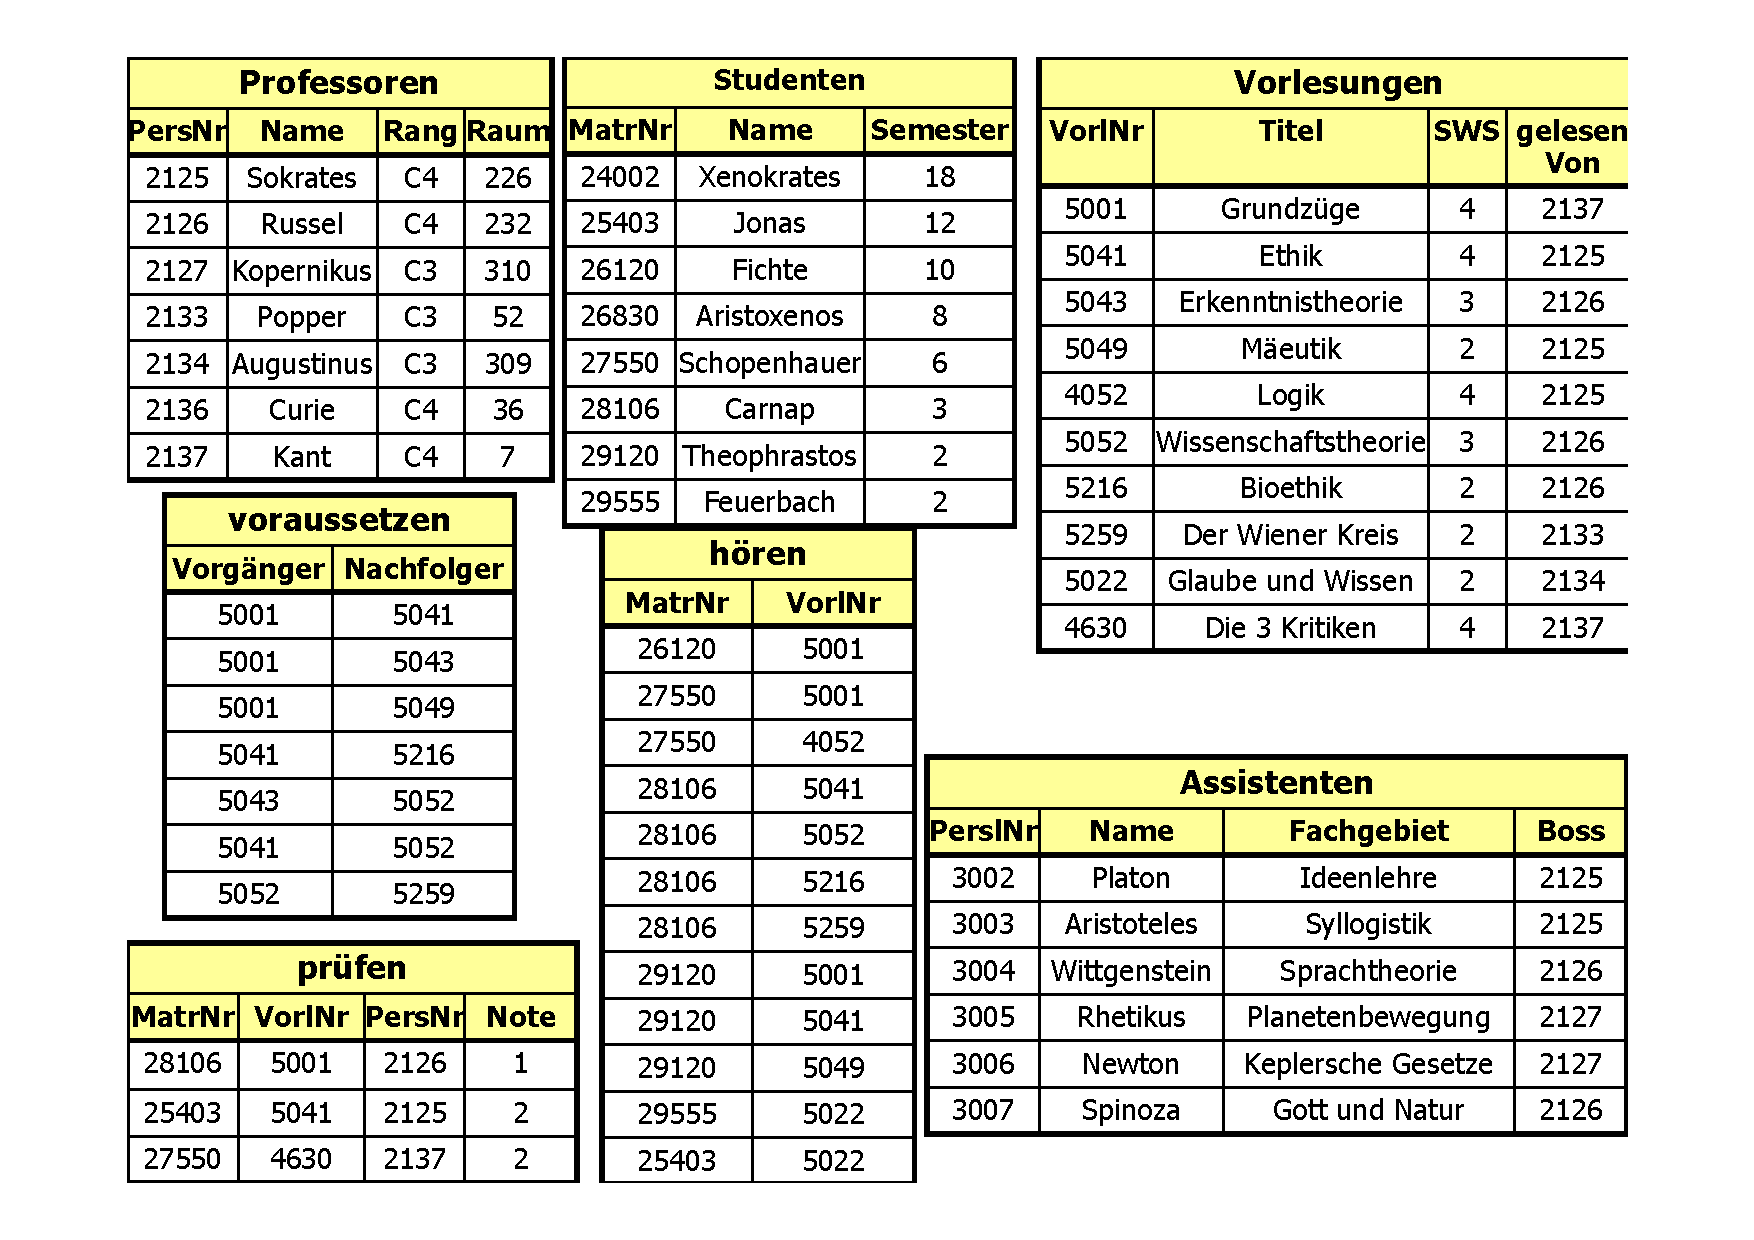
\includegraphics[height=.6\paperheight]{../img/uni.pdf}
		\end{center}
	\end{multicols}
\end{frame}

\begin{frame}[fragile]
	\frametitle{Hausaufgabe 2}
	\vspace{0.25cm}

	\begin{multicols}{2}
		Formulieren Sie die folgenden Anfragen auf dem bekannten Unischema in SQL:
		\begin{enumerate}[a)]
			% \item Bestimmen Sie das durchschnittliche Semester der Studenten der Universität.
			\item Bestimmen Sie das durchschnittliche Semester der Studenten, die mindestens eine Vorlesung bei Sokrates hören.
			% \item Bestimmen Sie, wie viele Vorlesungen im Schnitt pro Student gehört werden. 
			% 	  Beachten Sie, dass Studenten, die keine Vorlesung hören, in das Ergebnis einfließen müssen.
		\end{enumerate}
		\begin{minted}{sql}
WITH vorlesungen_von_sokrates as (
	SELECT * 
	FROM Vorlesungen v, Professoren p
	WHERE v.gelesenVon = p.PersNr
	  AND p.Name = 'Sokrates'
),
		\end{minted}
		\vfill\columnbreak

		\begin{minted}{sql}
studenten_von_sokrates as (
	SELECT * 
	FROM Studenten s
	WHERE EXISTS (
		SELECT *
		FROM hoeren h, 
		     vorlesungen_von_sokrates v
		WHERE h.MatrNr = s.MatrNr
		  AND v.VorlNr = h.VorlNr
	)
)
SELECT avg(Semester) FROM studenten_von_sokrates
		\end{minted}
	\end{multicols}
\end{frame}

\begin{frame}[fragile]
	\frametitle{Hausaufgabe 2 - Alternativlösung}
	\vspace{0.25cm}

	\begin{multicols}{2}
		Formulieren Sie die folgenden Anfragen auf dem bekannten Unischema in SQL:
		\begin{enumerate}[a)]
			\setcounter{enumi}{1}
			% \item Bestimmen Sie das durchschnittliche Semester der Studenten der Universität.
			\item Bestimmen Sie das durchschnittliche Semester der Studenten, die mindestens eine Vorlesung bei Sokrates hören.
			% \item Bestimmen Sie, wie viele Vorlesungen im Schnitt pro Student gehört werden. 
			% 	  Beachten Sie, dass Studenten, die keine Vorlesung hören, in das Ergebnis einfließen müssen.
		\end{enumerate}
		\begin{minted}{sql}
WITH vorlesungen_von_sokrates as (
	SELECT * 
	FROM Vorlesungen v, Professoren p
	WHERE v.gelesenVon = p.PersNr
	  AND p.Name = 'Sokrates'
),
		\end{minted}
		\vfill\columnbreak

		\begin{minted}{sql}
studenten_von_sokrates as (
	SELECT DISTINCT *
	FROM Studenten s, hoeren h, 
		 vorlesungen_von_sokrates v
	WHERE h.MatrNr = s.MatrNr 
	  AND v.VorlNr = h.VorlNr
)




SELECT avg(Semester) FROM studenten_von_sokrates
		\end{minted}
	\end{multicols}
\end{frame}

\begin{frame}[fragile]
	\frametitle{Hausaufgabe 2 - Alternativlösung}
	\vspace{0.25cm}

	\begin{multicols}{2}
		Formulieren Sie die folgenden Anfragen auf dem bekannten Unischema in SQL:
		\begin{enumerate}[a)]
			\setcounter{enumi}{2}
			% \item Bestimmen Sie das durchschnittliche Semester der Studenten der Universität.
			% \item Bestimmen Sie das durchschnittliche Semester der Studenten, die mindestens eine Vorlesung bei Sokrates hören.
			\item Bestimmen Sie, wie viele Vorlesungen im Schnitt pro Student gehört werden. 
				  Beachten Sie, dass Studenten, die keine Vorlesung hören, in das Ergebnis einfließen müssen.
		\end{enumerate}
		\vfill\columnbreak

		\begin{center}
			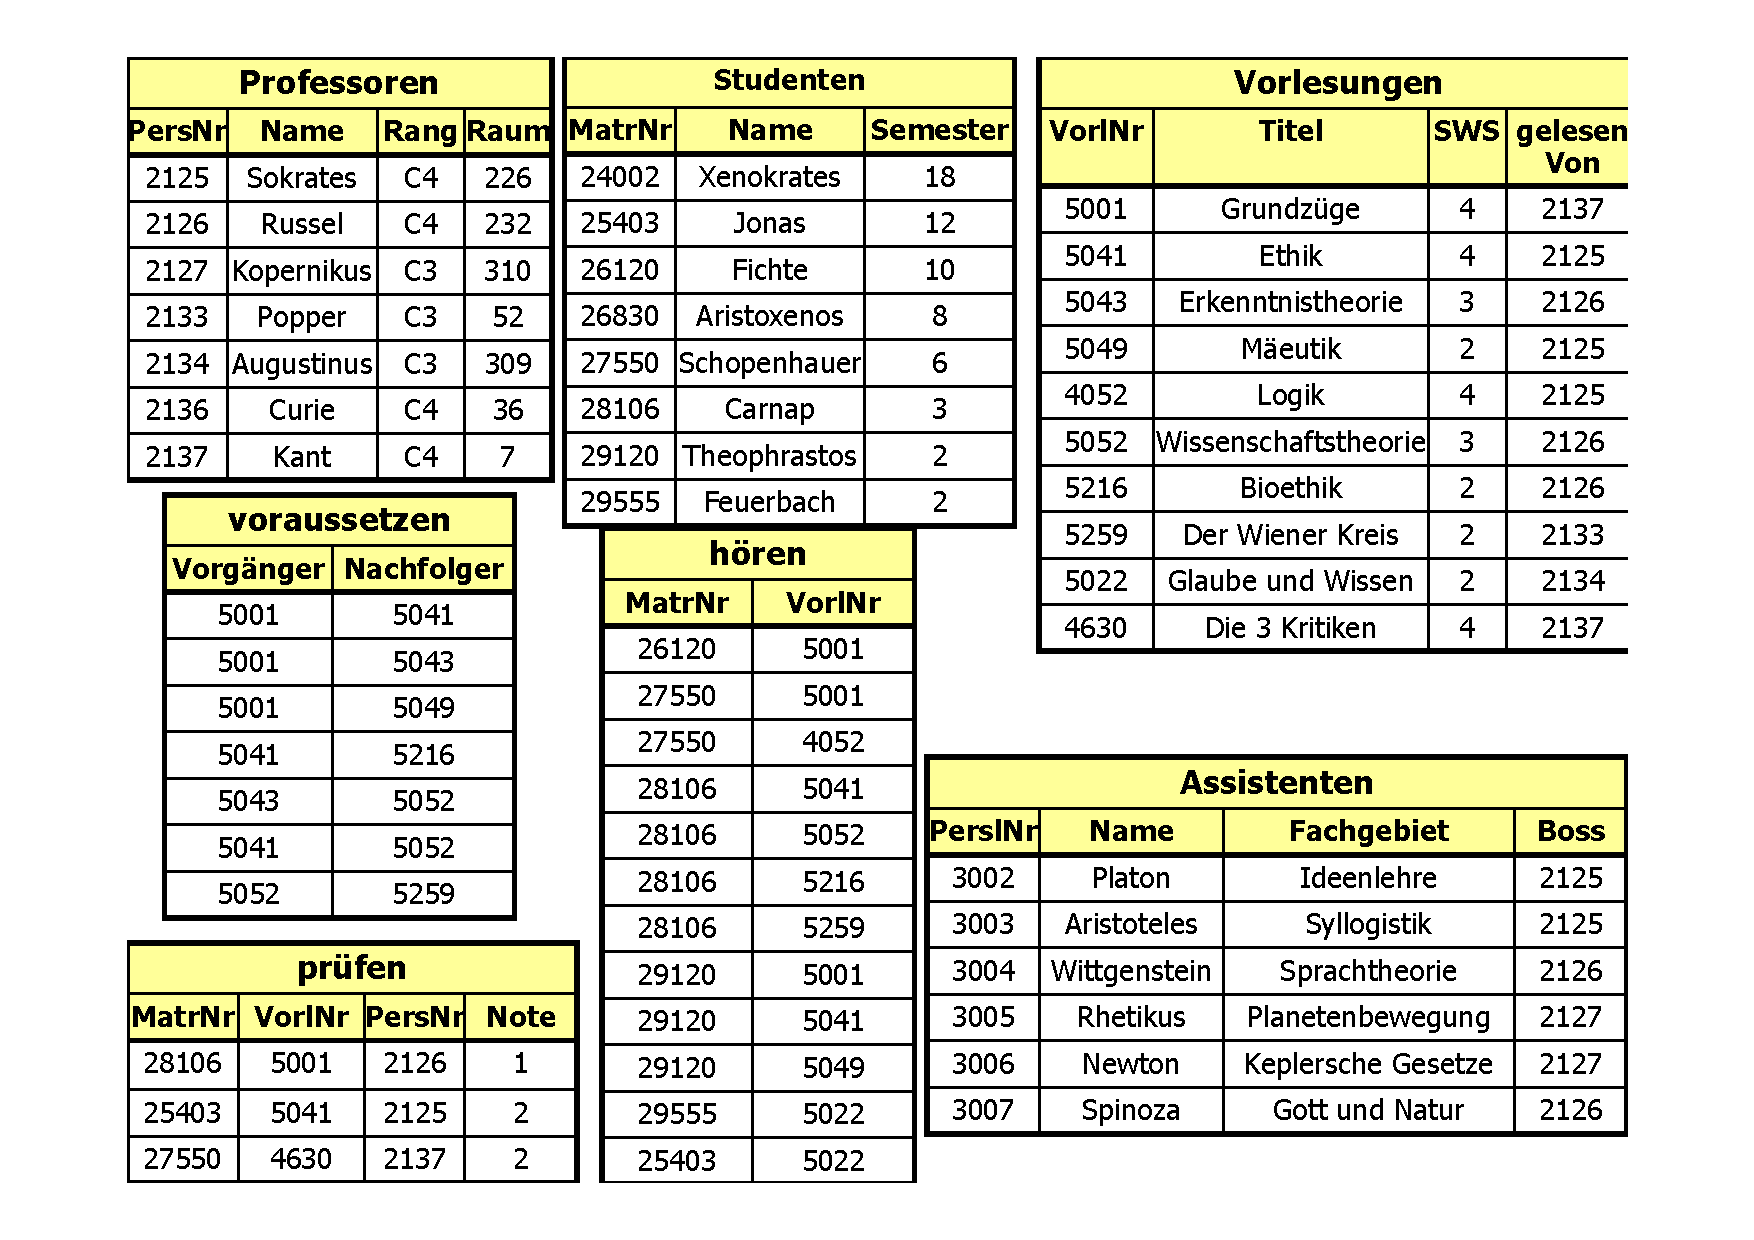
\includegraphics[height=.6\paperheight]{../img/uni.pdf}
		\end{center}
	\end{multicols}
\end{frame}

\begin{frame}[fragile]
	\frametitle{Hausaufgabe 2}
	\vspace{0.25cm}

	\begin{multicols}{2}
		Formulieren Sie die folgenden Anfragen auf dem bekannten Unischema in SQL:
		\begin{enumerate}[a)]
			\setcounter{enumi}{2}
			% \item Bestimmen Sie das durchschnittliche Semester der Studenten der Universität.
			% \item Bestimmen Sie das durchschnittliche Semester der Studenten, die mindestens eine Vorlesung bei Sokrates hören.
			\item Bestimmen Sie, wie viele Vorlesungen im Schnitt pro Student gehört werden. 
				  Beachten Sie, dass Studenten, die keine Vorlesung hören, in das Ergebnis einfließen müssen.
		\end{enumerate}
		\begin{minted}{sql}
SELECT hcount / (scount * 1.000)
FROM (SELECT count(*) AS hcount FROM hoeren) h,
     (SELECT count(*) AS scount FROM Studenten) s

SELECT hcount / (cast scount as decimal(10, 4))
FROM (SELECT count(*) AS hcount FROM hoeren) h,
     (SELECT count(*) AS scount FROM Studenten) s
		\end{minted}
		\vfill\columnbreak

		\begin{center}
			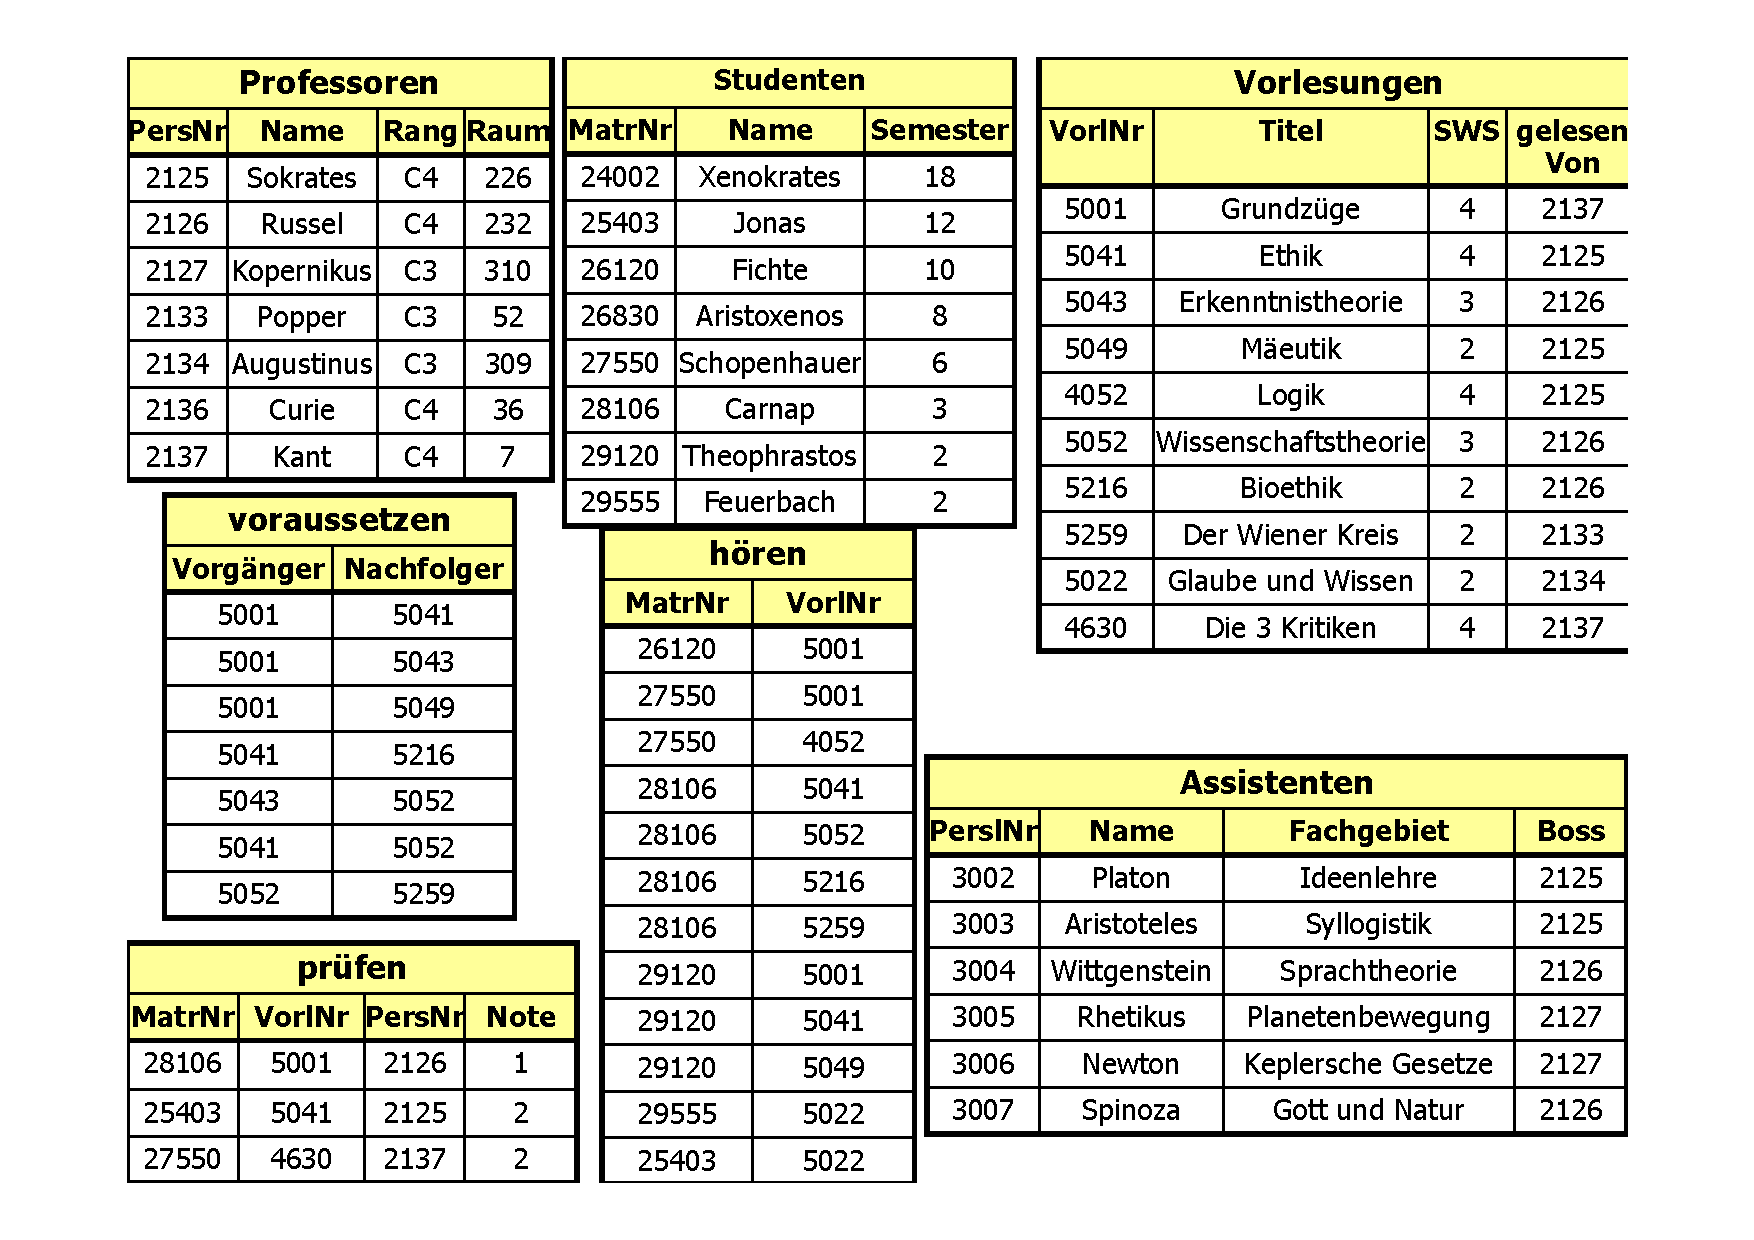
\includegraphics[height=.6\paperheight]{../img/uni.pdf}
		\end{center}
	\end{multicols}
\end{frame}

\begin{frame}[fragile]
	\frametitle{Hausaufgabe 3}
	\vspace{0.25cm}

	\begin{multicols}{2}
		Formulieren Sie eine SQL-Anfrage, um den Bekanntheitsgrad von Studenten zu ermitteln. \\
		Studenten kennen sich aus gemeinsam besuchten Vorlesungen.
		Ergebnis absteigend nach Bekanntheitsgrad sortieren
		\vfill\columnbreak

		\begin{center}
			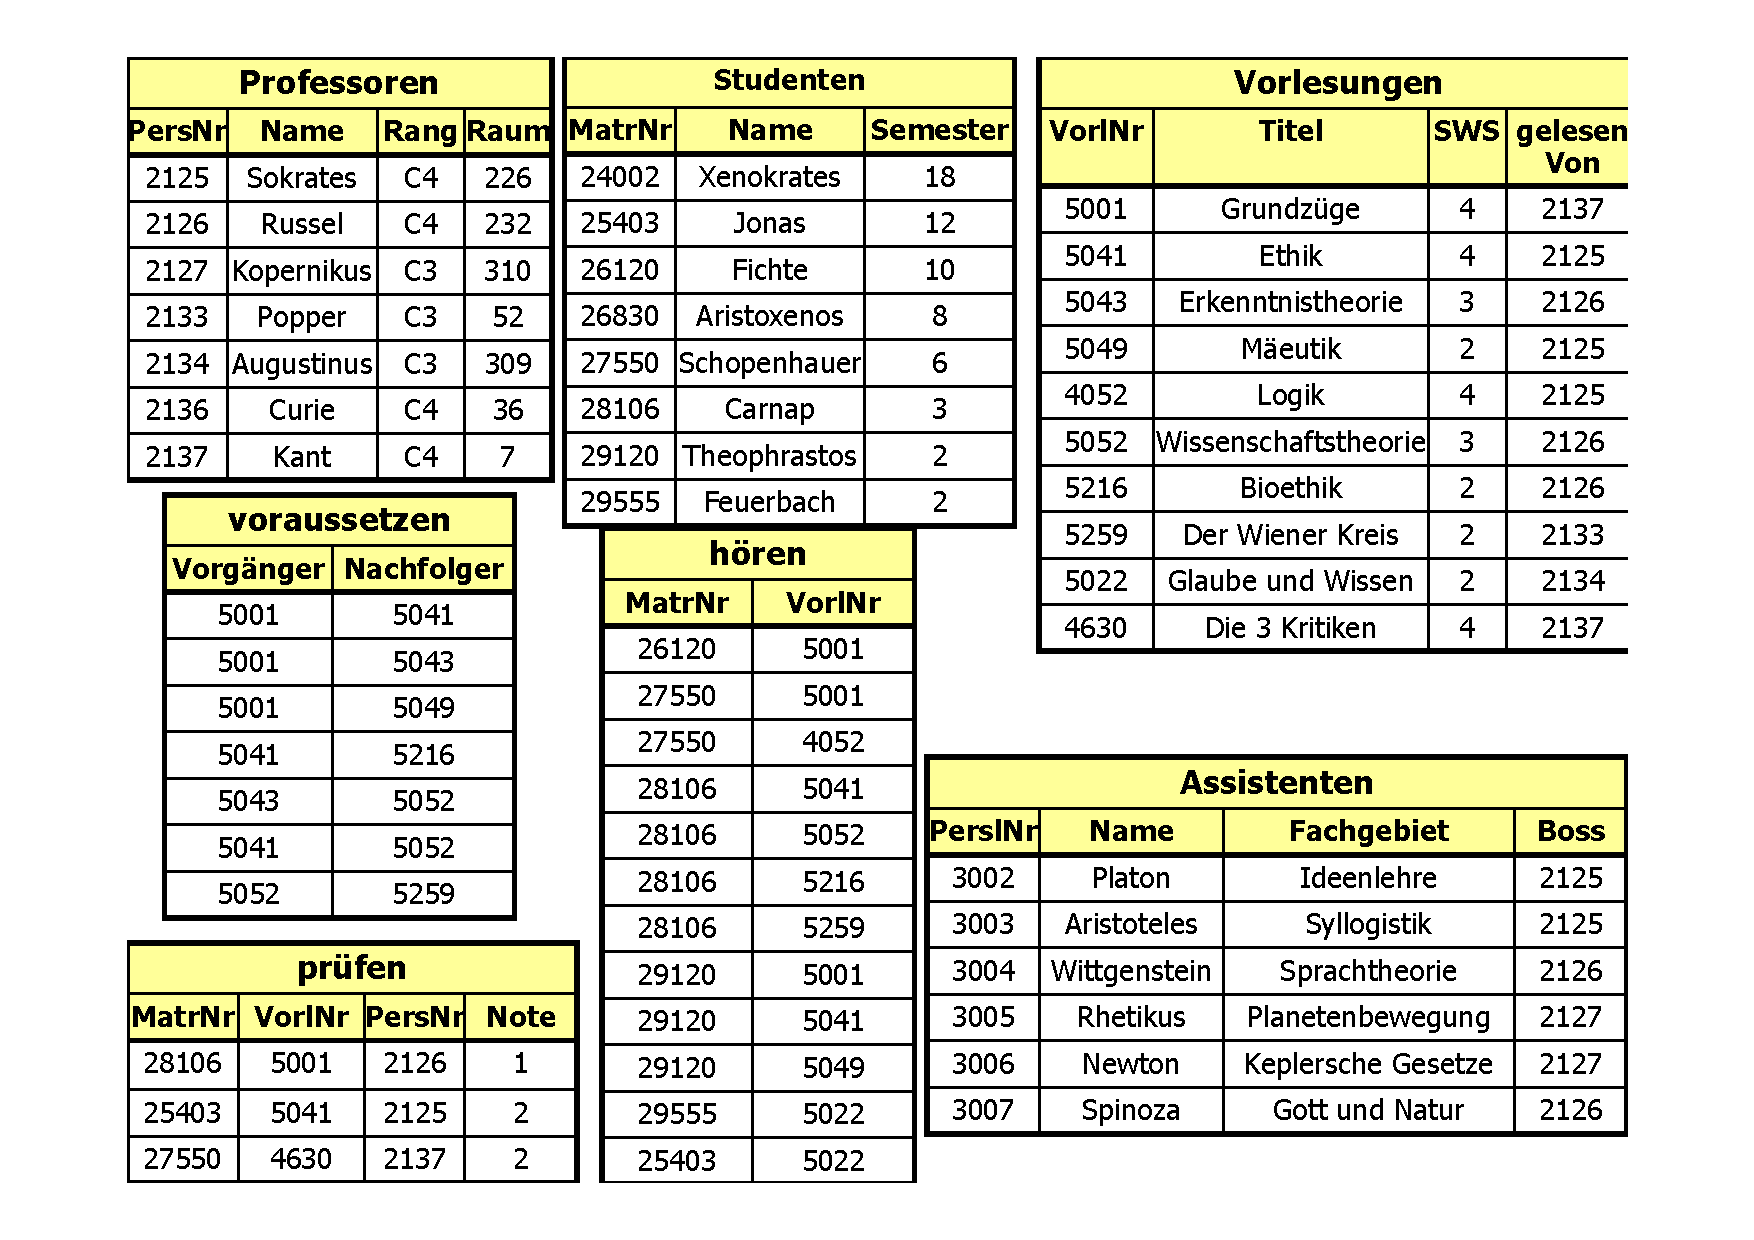
\includegraphics[height=.6\paperheight]{../img/uni.pdf}
		\end{center}
	\end{multicols}
\end{frame}

\begin{frame}[fragile]
	\frametitle{Hausaufgabe 3}
	\vspace{0.25cm}

	\begin{multicols}{2}
		Formulieren Sie eine SQL-Anfrage, um den Bekanntheitsgrad von Studenten zu ermitteln. \\
		Studenten kennen sich aus gemeinsam besuchten Vorlesungen.
		Ergebnis absteigend nach Bekanntheitsgrad sortieren

		\begin{minted}{sql}
WITH Bekannte AS (
	SELECT DISTINCT h1.MatrNr as Student,
	                h2.MatrNr AS Bekannter
	FROM hoeren h1, hoeren h2
	WHERE h1.VorlNr = h2.VorlNr
	  AND h2.MatrNr <> h1.MatrNr
)
		\end{minted}
		\vfill\columnbreak
		\begin{minted}{sql}
SELECT s.MatrNr, s.Name count(*) AS AnzBekannter
FROM Studenten s, (
	SELECT DISTINCT h1.MatrNr AS Student, 
	                 h2.MatrNr as Bekannter
	FROM hoeren h1, hoeren h2
	WHERE h1.VorlNr = h2.VorlNr
	  AND h2.MatrNr <> h1.MatrNr
	) b
WHERE s.MatrNr = b.Student
GROUP BY s.MatrNr, s.Name
ORDER BY AnzBekannter DESC;
		\end{minted}
	\end{multicols}
\end{frame}

\begin{frame}[fragile]
	\frametitle{Hausaufgabe 4}
	\vspace{0.25cm}

	\begin{multicols}{2}
		Gegeben sei die folgende (erweiterte) Relation ZehnkampfD mit 
		Athletennamen und den von ihnen erreichten Punkten in den jeweiligen Zehnkampfdisziplinen:

		\[ ZehnkampfD: \{[ \underline{Name, Disziplin}, Punkte ]\} \]

		Finden Sie alle ZehnkämpferInnen, die in \textit{allen} Disziplinen besser sind,
		als der Athlet \textit{Bolt} in
		\begin{itemize}
			\item relationaler Algebra
			\item relationalem Tupelkalkül
			\item relationalem Domänenkalkül
			\item SQL
		\end{itemize}
		\vfill\columnbreak

		\begin{table}[]
			\begin{tabular}{c|c|c}
				Name         & Disziplin    & Punkte      \\ \hline
				Eaton        & 100 m        & 450         \\
				Eaton        & Speerwurf    & 420         \\
				\( \hdots \) & \( \hdots \) & \( \hdots\) \\
				Eaton        & Weitsprung   & 420         \\
				Suarez       & 100 m        & 850         \\
				Suarez       & Speerwurf    & 620         \\
				\( \hdots \) & \( \hdots \) & \( \hdots\) \\
			\end{tabular}
		\end{table}
	\end{multicols}
\end{frame}

\begin{frame}[fragile]
	\frametitle{Hausaufgabe 4}
	\vspace{0.25cm}

	\begin{multicols}{2}
		Gegeben sei die folgende (erweiterte) Relation ZehnkampfD mit 
		Athletennamen und den von ihnen erreichten Punkten in den jeweiligen Zehnkampfdisziplinen:

		\[ ZehnkampfD: \{[ \underline{Name, Disziplin}, Punkte ]\} \]

		Finden Sie alle ZehnkämpferInnen, die in \textit{allen} Disziplinen besser sind,
		als der Athlet \textit{Bolt} in
		\begin{itemize}
			\item relationaler Algebra
			% \item relationalem Tupelkalkül
			% \item relationalem Domänenkalkül
			% \item SQL
		\end{itemize}
		\vfill\columnbreak

		\begin{center}
			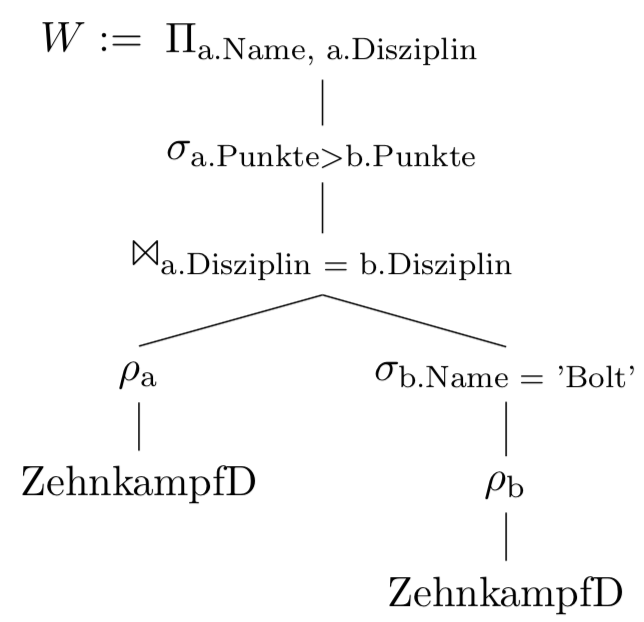
\includegraphics[height=.4\paperheight]{./4-a-1.png}
		\end{center}
		\pause 
		\begin{center}
			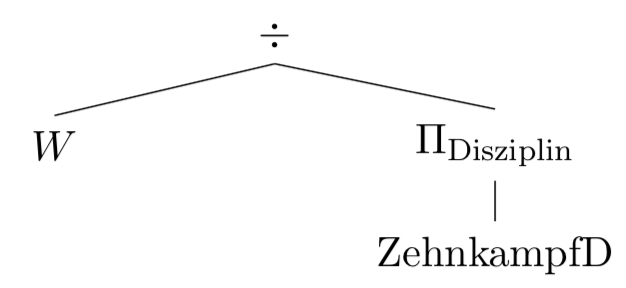
\includegraphics[height=.2\paperheight]{./4-a-2.png}
		\end{center}
	\end{multicols}
\end{frame}

\begin{frame}[fragile]
	\frametitle{Hausaufgabe 4}
	\vspace{0.25cm}

	\begin{multicols}{2}
		Gegeben sei die folgende (erweiterte) Relation ZehnkampfD mit 
		Athletennamen und den von ihnen erreichten Punkten in den jeweiligen Zehnkampfdisziplinen:

		\[ ZehnkampfD: \{[ \underline{Name, Disziplin}, Punkte ]\} \]

		Finden Sie alle ZehnkämpferInnen, die in \textit{allen} Disziplinen besser sind,
		als der Athlet \textit{Bolt} in
		\begin{itemize}
			% \item relationaler Algebra
			\item relationalem Tupelkalkül
			% \item relationalem Domänenkalkül
			% \item SQL
		\end{itemize}
		\vfill\columnbreak

		\begin{align*}
			\{ [a.Name] | & a \in ZehnkampfD \wedge \\
						  & \forall a' \in ZehnkampfD(a'.Name = a.Name) \\
						  & \Rightarrow \\
						  & \neg \exists b \in ZehnkampfD (b.Disziplin = a'.Disziplin \\
						  & \wedge b.Name = 'Bolt') \\
						  & \wedge b.Punkte \geq a'.Punkte) \\
			) \}
		\end{align*}
	\end{multicols}
\end{frame}

\begin{frame}[fragile]
	\frametitle{Hausaufgabe 4}
	\vspace{0.25cm}

	\begin{multicols}{2}
		Gegeben sei die folgende (erweiterte) Relation ZehnkampfD mit 
		Athletennamen und den von ihnen erreichten Punkten in den jeweiligen Zehnkampfdisziplinen:

		\[ ZehnkampfD: \{[ \underline{Name, Disziplin}, Punkte ]\} \]

		Finden Sie alle ZehnkämpferInnen, die in \textit{allen} Disziplinen besser sind,
		als der Athlet \textit{Bolt} in
		\begin{itemize}
			% \item relationaler Algebra
			% \item relationalem Tupelkalkül
			\item relationalem Domänenkalkül
			% \item SQL
		\end{itemize}
		\vfill\columnbreak

		\begin{align*}
			\{ [a] | & \exists d,p ([a, d, p] \in ZehnkampfD \wedge \\
					 & \forall d', p' ([a, d', p'] \in ZehnkampfD \\
					 & \Rightarrow \\
					 & \neg \exists bp (['Bolt', d', bp] \in ZehnkampfD \wedge bp \geq p') \\
					) \\
			)
			 \}
		\end{align*}
	\end{multicols}
\end{frame}

\begin{frame}[fragile]
	\frametitle{Hausaufgabe 4}
	\vspace{0.25cm}

	\begin{multicols}{2}
		Gegeben sei die folgende (erweiterte) Relation ZehnkampfD mit 
		Athletennamen und den von ihnen erreichten Punkten in den jeweiligen Zehnkampfdisziplinen:

		\[ ZehnkampfD: \{[ \underline{Name, Disziplin}, Punkte ]\} \]

		Finden Sie alle ZehnkämpferInnen, die in \textit{allen} Disziplinen besser sind,
		als der Athlet \textit{Bolt} in
		\begin{itemize}
			% \item relationaler Algebra
			% \item relationalem Tupelkalkül
			% \item relationalem Domänenkalkül
			\item SQL
		\end{itemize}
		\vfill\columnbreak
		Übersetzt aus der Anfrage im Tupelkalkül mit aufgelöstem \\
		\( \forall \)-Quantor und \( \Rightarrow \)
		\begin{minted}{sql}
SELECT DISTINCT a.Name from ZehnkampfD as a
WHERE NOT EXISTS (
	SELECT *
	FROM ZehnkampfD as a2
	WHERE a2.Name = a.Name
	  AND EXISTS (
		  SELECT *
		  FROM ZehnkampfD as b
		  WHERE b.Disziplin = a2.Disziplin
		    AND b.Name = 'Bolt'
		    AND b.Punkte >= a2.Punkte
	  )
)
		\end{minted}
	\end{multicols}
\end{frame}

\begin{frame}[fragile]
	\frametitle{Hausaufgabe 4}
	\vspace{0.25cm}

	\begin{multicols}{2}
		Gegeben sei die folgende (erweiterte) Relation ZehnkampfD mit 
		Athletennamen und den von ihnen erreichten Punkten in den jeweiligen Zehnkampfdisziplinen:

		\[ ZehnkampfD: \{[ \underline{Name, Disziplin}, Punkte ]\} \]

		Finden Sie alle ZehnkämpferInnen, die in \textit{allen} Disziplinen besser sind,
		als der Athlet \textit{Bolt} in
		% \begin{itemize}
		% 	% \item relationaler Algebra
		% 	% \item relationalem Tupelkalkül
		% 	% \item relationalem Domänenkalkül
		% 	\item SQL
		% \end{itemize}
		\begin{minted}{sql}
WITH disziplinen(anzahl) as (
	SELECT count(DISTINCT disziplin) AS anzahl
	FROM ZehnkampfD
),
		\end{minted}
		\vfill\columnbreak
		Alternative Formulierung mit Zählen der Tupel
		\begin{minted}{sql}
besserAlsBolt(name, disziplin) AS (
	SELECT a.Name, a.Disziplin
	FROM ZehnkampfD a, ZehnkampfD b
	WHERE b.name = 'Bolt'
	  AND a.Disziplin = b.Disziplin
	  AND a.Punkt > b.Punkte
)
SELECT Name 
FROM besserAlsBolt
GROUP BY name
HAVING count(*) = (
	SELECT anzahl FROM disziplinen
)
		\end{minted}
	\end{multicols}
\end{frame}
%%%%%%%%%%%%%%%%%%%%%%%%%%%%%%%%%%%%%%%%%%%%%%%%%%%%%%%%%%%%%%%%%%%%%%%%%%%%%%%%
\end{document} % !!! NICHT ENTFERNEN !!!
%%%%%%%%%%%%%%%%%%%%%%%%%%%%%%%%%%%%%%%%%%%%%%%%%%%%%%%%%%%%%%%%%%%%%%%%%%%%%%%%
